%% manuscript.tex
%% A Unified Homotopy Framework for Nonlinear System Identification and Simulation
%% Submitted to: Applied Mathematics and Computation (Elsevier)
%% Authors: R. H. Rodrigo, H. D. Patiño
%% Format: elsarticle, preprint, double-spaced, single-column
%% Revision: Improved version with multi-dimensional cases, noise robustness,
%%           and expanded optimizer comparisons

\documentclass[preprint,12pt,numbers]{elsarticle}

\usepackage{amsmath,amssymb,amsfonts,amsthm}
\usepackage{mathtools}
\usepackage{booktabs}
\usepackage{array}
\usepackage[table]{xcolor}
\usepackage{hyperref}
\usepackage{graphicx}
\usepackage{lineno}
\usepackage{url}
\usepackage{enumitem}

\graphicspath{{../figures/}{./figures/}}

\definecolor{lightgray}{RGB}{245,245,245}
\hypersetup{colorlinks=true, linkcolor=blue, citecolor=blue, urlcolor=blue}

\newcolumntype{L}[1]{>{\raggedright\arraybackslash}p{#1}}
\newcolumntype{C}[1]{>{\centering\arraybackslash}p{#1}}

\newtheorem{theorem}{Theorem}
\newtheorem{proposition}[theorem]{Proposition}
\newtheorem{corollary}[theorem]{Corollary}
\newtheorem{lemma}[theorem]{Lemma}
\newtheorem{definition}[theorem]{Definition}
\newtheorem{remark}[theorem]{Remark}

\usepackage[T1]{fontenc}

\journal{Applied Mathematics and Computation}

\begin{document}

\begin{frontmatter}

\title{A Unified Homotopy Framework for Nonlinear System Identification and Simulation:\\
Constructive Dimensioning of Bilinear Neural Architectures}

\author[inaut]{Rodolfo H. Rodrigo\corref{cor1}}
\ead{rrodrigo@inaut.unsj.edu.ar}
\cortext[cor1]{Corresponding author}

\author[inaut]{H. Daniel Pati\~no}
\ead{dpatino@inaut.unsj.edu.ar}

\affiliation[inaut]{organization={Instituto de Autom\'atica (INAUT), UNSJ--CONICET},
            addressline={Av. Libertador San Mart\'in (Oeste) 1109},
            city={San Juan},
            postcode={J5400ARL},
            state={San Juan},
            country={Argentina}}

\begin{abstract}
We develop a unified algorithmic framework for nonlinear system identification
and forward simulation of ordinary differential equations, built on Liao's
zeroth-order homotopy deformation equation. Both computational tasks---fitting
a parametric function approximator from input--output data, and
forward-integrating the resulting nonlinear ODE---are reduced to closed-form
Newton ($z_1$) and Halley ($z_2$) corrections derived from the same deformation
equation. The framework exploits the bilinear parameter structure of common
function representations (radial basis functions, sigmoid multilayer perceptrons):
a linear last-layer that admits an exact one-step least-squares solution, and
nonlinear internal parameters that admit curvature-aware corrections without
a scalar learning rate.

The principal theoretical contribution is a constructive dimensioning chain
$\varepsilon_{\mathrm{sim}} \to \varepsilon_{\mathrm{id}} \to M_{\min} \to N_{\min} \to T_{\max}$
that maps a target forward-simulation accuracy to the minimum number of basis
functions, the minimum number of training samples, and the maximum admissible
integration time step. The chain is constructive in the sense that each link is
computable from approximation-theoretic bounds and system quantities. An operator-theoretic
interpretation emerges: the choice of the auxiliary linear operator $\mathcal{L}$
encodes prior knowledge that reduces the residual nonlinearity the approximator
must learn, and therefore reduces the required approximator dimension.

We validate the framework on benchmark problems: a one-dimensional discharge-flow
system (orifice-tank model), a two-dimensional Lotka-Volterra predator-prey
system, and robustness experiments under measurement noise. Gaussian RBF and
sigmoid MLP approximators identified from sparse data (20--40 points) attain
identification residuals from $3\cdot 10^{-2}$ (RBF) down to machine precision
($1.7\cdot 10^{-8}$, MLP) in a single outer iteration and yield forward-simulation
errors of at most 2.3\% over 200-step horizons on the 1D benchmark. The scope of the empirical validation is
deliberately narrow---low-dimensional ODEs, small-scale approximators---and the
role of the present work is to establish the algorithmic framework, the
dimensioning theory, and the proof-of-concept computational regime; broader
empirical assessment and extension to high-dimensional or stiff systems are
identified as follow-up work.
\end{abstract}

\begin{keyword}
Homotopy analysis method \sep
nonlinear system identification \sep
ordinary differential equations \sep
radial basis functions \sep
Newton--Halley corrections \sep
constructive dimensioning \sep
bilinear approximation \sep
function approximation theory \sep
computational methods
\end{keyword}

\end{frontmatter}

\linenumbers

%% ======================================================================
\section{Introduction}
\label{sec:intro}
%% ======================================================================

Consider a nonlinear dynamical system observed through input--output data,
\begin{equation}
\dot{y}(t) + f(y(t)) = u(t), \qquad y(0) = y_0,
\label{eq:ode}
\end{equation}
where $f$ is an unknown nonlinearity and $u(t)$ is a measured excitation.
Two classical computational problems arise: \emph{identification}---reconstruct
$f$ from data $\{(t_i, y_i, u_i)\}_{i=1}^{N}$ using a parametric function
approximator---and \emph{forward simulation}---given an identified $\hat{f}$,
integrate \eqref{eq:ode} forward for new inputs and initial conditions. The two
are usually attacked with separate computational machinery. Identification employs
gradient-based optimization of parametric approximators (radial basis functions,
multilayer perceptrons \cite{Haykin2009,Park1991,Sjoberg1995,Nelles2001}) or,
more recently, sparse symbolic regression \cite{BruntonProctorKutz2016,Champion2019}.
Simulation employs explicit and implicit time-stepping schemes
\cite{Hairer1993,Butcher2016}. Each approach has its own convergence theory,
tuning parameters, and failure modes.

This paper isolates an algebraic structure that is common to both problems
and exploits it for joint, hyperparameter-light treatment. The starting
point is the zeroth-order deformation equation of the Homotopy Analysis
Method \cite{Liao2003,Liao2012,Liao2010},
\begin{equation}
(1-q)\,\mathcal{L}\!\left[\phi(q) - \phi_0\right] = q\,c_0\,\mathcal{N}[\phi(q)],
\qquad q \in [0,1],
\label{eq:deformation}
\end{equation}
in which $\mathcal{L}$ is a chosen linear operator, $\phi_0$ is an initial
approximation, and $c_0$ is a convergence-control parameter. Equation
\eqref{eq:deformation} is agnostic to the nature of $\phi$ and $\mathcal{N}$:
$\phi$ may be a parameter vector and $\mathcal{N}$ an approximation
residual, or $\phi$ may be a state trajectory and $\mathcal{N}$ a discretised
ODE residual. Truncating the homotopy series and matching powers of $q$
yields three closed-form corrections $z_1, z_2, z_3$ whose algebraic shape
depends only on the local Taylor coefficients of $\mathcal{N}$ at $\phi_0$,
not on the dimension or interpretation of $\phi$.

\paragraph{Contributions} The main contributions are the following.

\begin{enumerate}[label=(C\arabic*),leftmargin=*]
\item \emph{Universal deformation algebra.} We show that the corrections
$z_1$ and $z_2$, when read off the deformation equation
\eqref{eq:deformation}, recover Newton's method (with the choice
$\lambda = \mathcal{N}'_0$, $\sigma = -1$, $z_2 = 0$) and Halley's
method as instances, and admit a parametric extension to arbitrary
$\lambda$. This places HAM, Newton, and Halley in a common scalar
parametrisation $(\gamma, \sigma)$ that is exploited uniformly across
identification, simulation, and the linear/nonlinear sub-problems
within identification.

\item \emph{Bilinear factorisation of identification.} For both RBF and MLP
approximators, the identification residual is linear in the last-layer
weights and nonlinear in the internal parameters. The framework solves
the linear sub-problem exactly in one step ($z_1$ with quadratic form,
$z_2 = z_3 = 0$ structurally) and applies homotopy corrections only to
the nonlinear sub-problem. This is a Variable-Projection-style separation
\cite{GolubPereyra1973,Sjolund2014} but with curvature-aware
corrections instead of gradient descent on the projected residual.

\item \emph{Derivative-free integral simulation.} For the simulation step
we recast \eqref{eq:ode} as a Volterra integral equation with
exponential kernel $K(t,s) = e^{-k(t-s)}$, where $k$ is the linearisation
of the identified nonlinearity at the operating point. The discrete
residual then has all coefficients of order $O(1)$ and contains no
$1/T$ factor; sensor noise is attenuated rather than amplified. The
homotopy corrections on this residual give per-step convergence in
1--2 evaluations.

\item \emph{Constructive dimensioning.} We give explicit conditions linking
target simulation error $\varepsilon_{\mathrm{sim}}$ to identification
error $\varepsilon_{\mathrm{id}}$ (Gronwall propagation), to the
minimum number of basis functions $M_{\min}$ (RBF approximation rate
\`a la Buhmann \citeyear{Buhmann2003}; Barron norm \citeyear{Barron1993}
for sigmoid MLPs), to the minimum number of training samples $N_{\min}$
(Jacobian conditioning), and to the maximum admissible step $T_{\max}$
(Newton convergence on the integral residual). The chain is
constructive in the sense that each link is computable from system
quantities and the others are determined.

\item \emph{Inductive bias as operator choice.} The dimensioning chain
shows that $M_{\min}$ depends not on $\|f''\|_\infty$ globally but on
$\|\tilde{f}''\|_\infty$, where $\tilde{f} = f - \mathcal{L}^{-1}[f]$
is the residual nonlinearity left after the linear operator absorbs
the part of $f$ that is already known. Better prior knowledge produces
a smaller $\tilde{f}$ and reduces the network size needed for a given
accuracy. This formalises a quantitative meaning of ``inductive bias''
that is operator-side rather than loss-side, in contrast to
Physics-Informed Neural Networks (PINNs) \cite{Raissi2019} where
physics enters the loss as a soft penalty.
\end{enumerate}

\paragraph{Scope of the empirical study} The numerical results in
Section~\ref{sec:experiments} cover a one-dimensional first-order ODE
(orifice-tank discharge) with two architectures (5-centre RBF, 8-unit
sigmoid MLP) and 20 training points. The role of these experiments is to
verify, in the simplest non-trivial setting, that the closed-form
corrections converge as predicted, that the linear/nonlinear separation
behaves as analysed, and that the dimensioning chain is consistent with
the observed network sizes. Generalisation to multi-dimensional, stiff,
or chaotic dynamics, and to convolutional, recurrent, or attention-based
architectures, is consistent with the bilinear structure but requires
follow-up work; we discuss this explicitly in
Section~\ref{sec:limitations}.

\paragraph{Outline} Section~\ref{sec:related} positions the contribution
against gradient-based training, Newton-type methods for neural networks,
PINNs and Neural ODEs, and symbolic regression.
Section~\ref{sec:universal} states the deformation equation and derives
the universal scalar corrections.
Section~\ref{sec:identification} develops the identification level for
RBF and MLP architectures.
Section~\ref{sec:simulation} develops the integral simulation level.
Section~\ref{sec:unification} states the unification result in compact
form. Section~\ref{sec:dimensioning} establishes the constructive
dimensioning chain. Section~\ref{sec:prior} interprets the chain as a
formalisation of inductive bias.
Section~\ref{sec:experiments} reports the numerical demonstrations.
Section~\ref{sec:limitations} delineates the empirical scope and
identifies follow-up work.
Section~\ref{sec:companion} clarifies the relationship to companion
manuscripts by the authors. Section~\ref{sec:conclusions} concludes.


%% ======================================================================
\section{Related work}
\label{sec:related}
%% ======================================================================

\paragraph{Gradient-based neural network training} Backpropagation
\cite{RumelhartHintonWilliams1986} computes the gradient of a scalar
loss with respect to all parameters in a single backward pass; first-order
methods such as stochastic gradient descent and Adam \cite{Adam2015}
then update the parameters via a learning-rate-scaled step in the
negative-gradient direction. The combination is the workhorse of modern
deep learning, but for the small networks and physically-interpretable
problems we consider here it has well-known disadvantages: a learning
rate must be tuned, convergence is at best linear in the loss, and the
quality of the final iterate depends on initialisation and stopping.

\paragraph{Newton-type and second-order methods for neural networks}
Second-order methods exploit curvature information through the Hessian
or an approximation thereof. \citet{BeckerLeCun1988} proposed a diagonal
Hessian update for MLPs. \citet{Martens2010} introduced Hessian-free
optimisation, which builds Newton steps via conjugate gradient on
Hessian-vector products. The K-FAC family \cite{MartensGrosse2015}
approximates the Hessian by a Kronecker-factored block-diagonal
structure. The framework of the present paper is closer in spirit to
\citet{Sjolund2014}, who exploit the linear/nonlinear separation of
single-hidden-layer networks via Variable Projection. The principal
differences are: (i) we derive the corrections $z_1, z_2$ from the
deformation equation rather than from a Levenberg--Marquardt or
Gauss--Newton starting point, which gives a uniform parametrisation
across identification and simulation; (ii) we apply the same
corrections to ODE simulation, not only to identification; and (iii)
we add an explicit dimensioning analysis that links the corrections'
convergence conditions to network size and data sufficiency.

\paragraph{Physics-Informed Neural Networks} PINNs
\cite{Raissi2019,KarniadakisEtAl2021} embed the governing differential
equation into a soft penalty in the training loss and minimise the
combined data-plus-physics loss with backpropagation. The architecture
is left untouched. Two consequences follow: (i) the network size must
be chosen heuristically because the physics term does not change the
function class, only the search direction; (ii) the loss landscape
becomes ill-conditioned when the physics weight is large or the system
is stiff \cite{WangPerdikaris2021,Krishnapriyan2021}. The framework of
the present paper places physics in the auxiliary linear operator
$\mathcal{L}$ and consequently in the residual nonlinearity
$\tilde{f} = f - \mathcal{L}^{-1}[f]$ that the network must approximate.
The effect on architecture is constructive: better prior knowledge
shrinks $\|\tilde{f}''\|_\infty$ and therefore the required $M$.

\paragraph{Neural Ordinary Differential Equations} \citet{ChenEtAl2018}
parametrise the right-hand side of an ODE by a neural network and train
it via the adjoint method. This is conceptually orthogonal to our work:
their primary problem is to back-propagate through the ODE solver
efficiently for general loss functions on the trajectory; our primary
problem is to identify $f$ from sparse data and then simulate accurately.
\citet{Rackauckas2020} unify these directions under the Universal
Differential Equations programme, where physics-known terms are
combined with neural-network-learned residual terms; that combination
is precisely the operator-side decomposition $f = \mathcal{L}^{-1}[\cdot] + \tilde{f}$
that we use here, and our dimensioning analysis applies to it.

\paragraph{Symbolic and sparse identification} SINDy
\cite{BruntonProctorKutz2016} and its extensions
\cite{Champion2019,Kaheman2020} reconstruct $f$ from data by sparse
regression on a candidate library of nonlinear basis functions, with
$\ell_1$-style penalties to enforce parsimony. The output is a symbolic
expression rather than a black-box approximator. Our framework is
intermediate between SINDy and classical neural identification: the
basis is a smooth parametrised family (RBF, MLP) rather than a fixed
library, but the linear sub-problem is solved exactly as in SINDy and
the nonlinear corrections are closed-form rather than gradient-based.

\paragraph{Reservoir computing and echo-state networks}
\citet{Lukosevicius2009} train only the linear output layer of a
recurrent network, freezing the nonlinear hidden dynamics. The
linear/nonlinear split is identical in spirit to the one we use,
restricted to the case in which the nonlinear part is fixed by design.
Our framework treats both halves: the linear part exactly, the nonlinear
part by curvature-aware corrections.

\paragraph{Homotopy methods in numerical analysis and control}
The Homotopy Analysis Method \cite{Liao2003,Liao2012} was developed for
analytic series solutions to nonlinear differential and integral
equations. \citet{Turkyilmazoglu2010} and \citet{VajraveluVanGorder2013}
analysed convergence properties and the role of the auxiliary parameter
$c_0$. Within optimisation, \citet{Allgower2003} reviewed numerical
continuation methods, of which homotopy is a special case. The
contribution of the present paper is to use the deformation equation as
an \emph{algorithmic} primitive---truncated, evaluated numerically, and
applied uniformly to identification and simulation---rather than as a
device for analytic series construction.


%% ======================================================================
\section{The universal deformation equation}
\label{sec:universal}
%% ======================================================================

\subsection{Liao's zeroth-order deformation}

Given a nonlinear operator $\mathcal{N}$ acting on an unknown $\phi$ with
$\mathcal{N}[\phi^*] = 0$, the deformation equation \eqref{eq:deformation}
constructs a one-parameter family $\phi(q)$, $q \in [0,1]$, such that
$\phi(0) = \phi_0$ and $\phi(1) = \phi^*$. The freedom in choosing
$\mathcal{L}$, $\phi_0$, and $c_0$ is the analytic content of the method
\cite{Liao2010}. We use this freedom algorithmically: $\mathcal{L}$
encodes prior knowledge, $\phi_0$ is the best available cheap
approximation, and $c_0$ scales the corrections.

\subsection{The universal scalar corrections}

Expanding $\phi(q) = \phi_0 + \sum_{m \geq 1} z_m\,q^m$ and Taylor-expanding
$\mathcal{N}[\phi_0 + \delta]$ about $\phi_0$, matching coefficients of
$q^m$ in \eqref{eq:deformation} yields, in scalar form,
\begin{equation}
\boxed{\;
z_1 = \gamma, \qquad
z_2 = \gamma(1+\sigma), \qquad
z_3 = \gamma(1+\sigma)^2 + \frac{c_0\,\mathcal{N}''_0}{2\,\lambda}\,\gamma^2,
\;}
\label{eq:z123}
\end{equation}
where
\begin{equation}
\gamma \triangleq \frac{c_0\,\mathcal{N}_0}{\lambda}, \qquad
\sigma \triangleq \frac{c_0\,\mathcal{N}'_0}{\lambda},
\label{eq:gamma-sigma}
\end{equation}
$\mathcal{N}_0 = \mathcal{N}[\phi_0]$, $\mathcal{N}'_0 = \partial\mathcal{N}/\partial\phi\big|_{\phi_0}$,
$\mathcal{N}''_0 = \partial^2\mathcal{N}/\partial\phi^2\big|_{\phi_0}$,
and $\lambda$ is the scalar representation of $\mathcal{L}$. For
finite-dimensional problems $\lambda$ is a chosen positive scalar; for
differential operators $\lambda$ incorporates the discretisation. The
truncated series converges if $|1+\sigma| < 1$, equivalently
$0 < \mathcal{N}'_0/\lambda < 2$ for $c_0 = -1$.

\begin{remark}[Newton and Halley as special cases]
With $\lambda = \mathcal{N}'_0$ and $c_0 = -1$ one obtains $\sigma = -1$,
hence $z_2 = 0$ and $z_3$ reduces to the classical Halley correction
$-\tfrac{1}{2}\mathcal{N}_0^2\,\mathcal{N}''_0/(\mathcal{N}'_0)^3$
\cite{Gutierrez1997}. The expressions \eqref{eq:z123} therefore
generalise Newton--Halley to arbitrary $\lambda$, with the
$\sigma$-parametrised one-parameter family interpolating between the
two and beyond.
\end{remark}

\begin{remark}[Vectorial reading]
For $\phi \in \mathbb{R}^n$, the scalar $\mathcal{N}'_0$ is replaced by a
Jacobian and $\mathcal{N}''_0$ by a Hessian tensor. With $\lambda = J^TJ$
(Gauss--Newton metric) and a diagonal Hessian approximation, the
expressions \eqref{eq:z123} produce the Levenberg--Marquardt step at
order one and a Halley-type correction at order two. The diagonal
Hessian approximation is a deliberate choice to retain $O(NM)$ cost per
step; we discuss its accuracy in Section~\ref{sec:identification}.
\end{remark}


%% ======================================================================
\section{Identification by homotopy}
\label{sec:identification}
%% ======================================================================

\subsection{Problem statement and bilinear factorisation}

We represent the unknown nonlinearity by a parametric approximator with
linear last layer,
\begin{equation}
\hat{f}(y) = \boldsymbol{\Phi}(y;\boldsymbol{\eta})\,\mathbf{w},
\label{eq:bilinear}
\end{equation}
where $\boldsymbol{\Phi}: \mathbb{R} \to \mathbb{R}^{1\times M}$ is a row of
basis functions parametrised by $\boldsymbol{\eta}$ (centres and widths
for an RBF; hidden weights and biases for an MLP), and
$\mathbf{w} \in \mathbb{R}^M$ are linear weights. Given training data
$\{(y_i, f_i)\}_{i=1}^N$, the identification residual is
\begin{equation}
\mathcal{N}_{\mathrm{id}}(\boldsymbol{\eta}, \mathbf{w}) =
\boldsymbol{\Phi}(\boldsymbol{\eta})\,\mathbf{w} - \mathbf{f},
\label{eq:Nid}
\end{equation}
where $\boldsymbol{\Phi}_{ij} = \boldsymbol{\Phi}(y_i;\boldsymbol{\eta})_j$
is the $N \times M$ design matrix and
$\mathbf{f} = (f_1, \ldots, f_N)^T$.

The residual is \emph{linear} in $\mathbf{w}$ and \emph{nonlinear} in
$\boldsymbol{\eta}$. We exploit this by alternating an exact linear solve
on $\mathbf{w}$ with curvature-aware corrections on $\boldsymbol{\eta}$.

\subsection{Linear sub-problem (last-layer weights)}

For fixed $\boldsymbol{\eta}$, the optimal weights are
\begin{equation}
\mathbf{w}^* = (\boldsymbol{\Phi}^T\boldsymbol{\Phi})^{-1}\boldsymbol{\Phi}^T\mathbf{f}.
\label{eq:ls}
\end{equation}
This is the deformation correction $z_1$ with $\mathcal{L} = \boldsymbol{\Phi}^T\boldsymbol{\Phi}$
applied to the linear residual; structurally,
$\partial^2\mathcal{N}_{\mathrm{id}}/\partial\mathbf{w}^2 = 0$, so
$z_2 = z_3 = 0$ and the solution is exact in one step.

\subsection{Nonlinear sub-problem (internal parameters)}

After substituting $\mathbf{w} = \mathbf{w}^*(\boldsymbol{\eta})$, the
residual is a function of $\boldsymbol{\eta}$ only. The Jacobian
$J_\eta$ is computed analytically; for an RBF with centre $c_j$ and
width $\lambda_j$,
\begin{align}
\frac{\partial\mathcal{N}_i}{\partial c_j} &=
w_j\,\varphi'\!\left(\frac{|y_i - c_j|}{\lambda_j}\right)\,\frac{\mathrm{sgn}(y_i - c_j)}{\lambda_j},
\\
\frac{\partial\mathcal{N}_i}{\partial\lambda_j} &=
-w_j\,\varphi'\!\left(\frac{|y_i - c_j|}{\lambda_j}\right)\,\frac{|y_i - c_j|}{\lambda_j^2}.
\end{align}
For an MLP the corresponding derivatives are obtained by analytical
differentiation of the activation, e.g.\ $\sigma'(x) = \sigma(x)(1-\sigma(x))$
and $\sigma''(x) = \sigma'(x)(1-2\sigma(x))$ for the logistic sigmoid.
We emphasise that these closed-form derivatives \emph{are} the
parameter-by-parameter chain rule and so are mathematically equivalent
to backpropagation; the difference is downstream of the gradient. We do
not use a learning rate or stochastic batches.

The Newton correction on the nonlinear parameters is
\begin{equation}
\Delta\boldsymbol{\eta}_1 = -(J_\eta^T J_\eta)^{-1}\,J_\eta^T\,\mathcal{N}_0,
\label{eq:z1-eta}
\end{equation}
which is $z_1$ of \eqref{eq:z123} read in vectorial form with
$\lambda = J_\eta^T J_\eta$. For the Halley correction we use a
\emph{diagonal} Hessian approximation,
\begin{equation}
\Delta\eta_{j,2} \approx -\tfrac{1}{2}\,\frac{(\mathcal{N}_1^T\,\partial^2\mathcal{N}/\partial\eta_j^2)\,(\Delta\eta_{j,1})^2}
{(J_{\eta j}^T J_{\eta j})},
\label{eq:z2-eta}
\end{equation}
where $\mathcal{N}_1$ is the residual after the Newton step.

\paragraph{Diagonal-Hessian approximation: scope and effect}
Equation \eqref{eq:z2-eta} retains only the $j$-diagonal entries of the
parameter Hessian. The exact Halley step contains additional off-diagonal
contributions that scale with the off-diagonal Hessian entries. The
diagonal approximation is exact when the Hessian is diagonally dominant
(in particular when the basis functions $\varphi_j$ have non-overlapping
supports relative to the data) and is otherwise a controlled approximation
that preserves quadratic convergence under the same conditions as Newton.
We use it because (i) it keeps the per-iteration cost at $O(NM)$ and
(ii) it is the form that survives the universal scalar parametrisation
\eqref{eq:z123}. For problems in which the basis functions overlap
strongly, a Kronecker-factored Hessian \cite{MartensGrosse2015} can
replace the diagonal in \eqref{eq:z2-eta} without changing the rest of
the framework.

\subsection{Algorithm}

Algorithm~\ref{alg:identification} states the identification procedure.

\begin{table}[h]
\centering
\caption{Identification algorithm (one outer iteration; iterate until
$\|\mathcal{N}\| < \varepsilon$).}
\label{alg:identification}
\begin{tabular}{rl}
\toprule
\textbf{Step} & \textbf{Action} \\
\midrule
1 & Initialise $\boldsymbol{\eta}^{(0)}$ (K-means for RBF; uniform grid for MLP). \\
2 & Solve $\mathbf{w}^* \leftarrow (\boldsymbol{\Phi}^T\boldsymbol{\Phi})^{-1}\boldsymbol{\Phi}^T\mathbf{f}$
    \quad ($z_1$ exact, one step). \\
3 & Form $J_\eta$ analytically; apply Newton step \eqref{eq:z1-eta}. \\
4 & Recompute $\mathbf{w}^*$ and the residual; apply Halley step \eqref{eq:z2-eta}. \\
5 & Recompute $\mathbf{w}^*$; check $\|\mathcal{N}\| < \varepsilon$. \\
\bottomrule
\end{tabular}
\end{table}


%% ======================================================================
\section{Simulation by integral homotopy}
\label{sec:simulation}
%% ======================================================================

\subsection{Operator splitting and analytic starting solution}

After identification, the simulation problem is to integrate
$\dot{y} + \hat{f}(y) = u(t)$ from $y(0) = y_0$. We linearise the
identified RHS at a reference point $\bar{y}$,
\begin{equation}
k = \hat{f}'(\bar{y}),
\qquad
\tilde{f}(y) = \hat{f}(y) - k\,y,
\end{equation}
so that $\tilde{f}'(\bar{y}) = 0$ by construction, and split
\begin{equation}
\dot{y} + k\,y = u(t) - \tilde{f}(y).
\label{eq:split}
\end{equation}
The left-hand side is a first-order linear operator with analytic Green's
function $K(t,s) = e^{-k(t-s)}$, yielding the starting solution
\begin{equation}
y_0(t) = y_0\,e^{-kt} + \int_0^t K(t,s)\,u(s)\,\mathrm{d}s.
\label{eq:y0}
\end{equation}

\subsection{Volterra integral residual}

Equation \eqref{eq:split} is equivalent to the Volterra integral equation
\begin{equation}
y(t) = y_0(t) - \int_0^t K(t,s)\,\tilde{f}(y(s))\,\mathrm{d}s.
\label{eq:volterra}
\end{equation}
Discretising the integral with the trapezoidal rule at step $T$ and
maintaining the convolution as an IIR accumulator $S_n$ with update
$S_n = e^{-kT}\,S_{n-1} + T\,w_n[u_n - \tilde{f}(y_n)]$ (where $w_n$ are
the trapezoidal weights), the per-step residual reads
\begin{equation}
g_{\mathrm{sim}}(y_n) = y_n + T\,w_n\,\tilde{f}(y_n)
- T\,w_n\,u_n
- e^{-kT}\,S_{n-1} - y_0\,e^{-k\,t_n}.
\label{eq:g-sim}
\end{equation}
The Jacobian $g'_{\mathrm{sim}} = 1 + T\,w_n\,\tilde{f}'(y_n)$ is $O(1)$
and contains no $1/T$ factor; sensor noise on $u$ is multiplied by $T$
rather than divided by $T$, which is the standard advantage of integral
formulations \cite{Atkinson1997,Kress2014}.

\subsection{Per-step homotopy correction}

The per-step deformation uses \eqref{eq:z123} with $\mathcal{N}_0 = g_{\mathrm{sim}}(y_n^{(0)})$,
$\mathcal{N}'_0 = g'_{\mathrm{sim}}$, $\mathcal{N}''_0 = T\,w_n\,\tilde{f}''(y_n)$,
and $\lambda = g'_{\mathrm{sim}}$. With this choice $\sigma = -1$,
$z_2 = 0$, and $z_3$ is the standard Halley correction. The cost is one
linear-system solve (scalar, in the SISO case) and three evaluations of
$\tilde{f}$ per step.


%% ======================================================================
\section{Unification: identification and simulation as one equation}
\label{sec:unification}
%% ======================================================================

\begin{table}[h]
\centering
\caption{Subproblems in the unified framework. Each row is an instance of
the deformation equation \eqref{eq:deformation} with the indicated
choice of $(\mathcal{L}, \mathcal{N}, \phi, \lambda)$.}
\label{tab:levels}
\rowcolors{2}{lightgray}{white}
\begin{tabular}{C{0.6cm} L{2.5cm} C{1.0cm} L{3.5cm} L{2.4cm} L{2.0cm}}
\toprule
\textbf{Level} & \textbf{Sub-problem} & $\boldsymbol{\mathcal{L}}$ & $\boldsymbol{\mathcal{N}}$ & $\boldsymbol{\phi}$ & $\boldsymbol{\lambda}$ \\
\midrule
1a & Last-layer weights & $\boldsymbol{\Phi}^T\boldsymbol{\Phi}$ & $\boldsymbol{\Phi}\mathbf{w} - \mathbf{f}$ & $\mathbf{w} \in \mathbb{R}^M$ & $\boldsymbol{\Phi}^T\boldsymbol{\Phi}$ \\
1b & Internal parameters & $J_\eta^T J_\eta$ & $\mathcal{N}_{\mathrm{id}}(\boldsymbol{\eta})$ & $\boldsymbol{\eta} \in \mathbb{R}^{2M}$ & $J_\eta^T J_\eta$ \\
2 & ODE forward step & $\mathrm{d}/\mathrm{d}t + k$ & $\dot{y} + \tilde{f}(y) - u$ & $y_n \in \mathbb{R}$ & $g'_{\mathrm{sim}}$ \\
\bottomrule
\end{tabular}
\end{table}

\begin{theorem}[Unified homotopy framework]\label{thm:unified}
The three sub-problems in Table~\ref{tab:levels} are instances of the
deformation equation \eqref{eq:deformation}, with corrections given by
the universal scalar formulae \eqref{eq:z123}. Specifically:
\begin{enumerate}[nosep]
\item[(i)]\hspace{0.5em}Level~1a is solved exactly in one step ($z_2 = z_3 = 0$ structurally).
\item[(ii)]\hspace{0.4em}Level~1b converges if $0 < \mathcal{N}'_0/\lambda < 2$ at each iterate, with
quadratic rate from $z_1$ alone and cubic rate from $z_1 + z_2$ when the
Hessian is diagonally dominant.
\item[(iii)]\hspace{0.2em}Level~2 converges per step if $\tilde{f}$ is Lipschitz and $T < 1/\max|\tilde{f}'|$.
\item[(iv)]\hspace{0.4em}No scalar learning rate or stochastic batching is used at any level.
\end{enumerate}
\end{theorem}

\begin{proof}[Proof sketch]
(i) Linearity of the residual in $\mathbf{w}$.
(ii) Standard Newton convergence with curvature correction; the
diagonal-dominance condition is sufficient for the diagonal Hessian
approximation to retain Halley's cubic rate.
(iii) Compactness of the Volterra operator implies convergence of the
Neumann series for finite horizons \cite{Kress2014}; the step-size
condition is the per-step Newton condition on the integral residual.
(iv) By construction.
\end{proof}

\subsection{Recovery of classical methods}

\begin{table}[h]
\centering
\caption{The framework recovers classical numerical methods as parameter
choices in \eqref{eq:z123}.}
\label{tab:connections}
\rowcolors{2}{lightgray}{white}
\begin{tabular}{L{4.0cm} L{3.5cm} L{4.5cm}}
\toprule
\textbf{Choice} & \textbf{Method recovered} & \textbf{Reference} \\
\midrule
$\mathcal{L} = \boldsymbol{\Phi}^T\boldsymbol{\Phi}$, $z_1$ on $\mathbf{w}$ &
Linear least squares & \citet{Bjorck1996} \\
$\mathcal{L} = J^TJ$, $z_1$ on $(\mathbf{w}, \boldsymbol{\eta})$ &
Variable Projection / Gauss--Newton & \citet{GolubPereyra1973,Sjolund2014} \\
$\mathcal{L} = J^TJ$, $z_1 + z_2$ scalar &
Halley's method & \citet{Gutierrez1997} \\
$\mathcal{L} = \mathrm{d}/\mathrm{d}t$, integral residual &
Picard iteration & \citet{Atkinson1997} \\
$\mathcal{L} = \mathrm{d}/\mathrm{d}t + k$, $z_1+z_2+z_3$ on integral residual &
\textbf{Integral Newton--Halley} & This paper, Section~\ref{sec:simulation} \\
\bottomrule
\end{tabular}
\end{table}


%% ======================================================================
\section{Constructive dimensioning}
\label{sec:dimensioning}
%% ======================================================================

We now derive the dimensioning chain.

\subsection{From simulation accuracy to identification accuracy}

\begin{theorem}[Gronwall propagation]\label{thm:propagation}
Let $y(t)$ solve $\dot{y} + f(y) = u$ and $\hat{y}(t)$ solve
$\dot{y} + \hat{f}(y) = u$ with the same initial condition. If $f$ is
Lipschitz with constant $L$ and $\|f - \hat{f}\|_\infty = \varepsilon_{\mathrm{id}}$,
then for $t \in [0, T_f]$,
\begin{equation}
\|y - \hat{y}\|_{\infty,[0,T_f]} \leq
\varepsilon_{\mathrm{id}}\,\frac{e^{L\,T_f} - 1}{L}.
\label{eq:gronwall}
\end{equation}
\end{theorem}
\begin{proof}
Standard Gronwall on $e(t) = y(t) - \hat{y}(t)$ with $|\dot{e}| \leq L|e| + \varepsilon_{\mathrm{id}}$.
\end{proof}

Inverting,
\begin{equation}
\varepsilon_{\mathrm{id}} \leq
\varepsilon_{\mathrm{sim}}\,\frac{L}{e^{L\,T_f} - 1}.
\label{eq:eps-id-required}
\end{equation}

\subsection{From identification accuracy to network size}

\begin{proposition}[RBF approximation rate, \citealp{Buhmann2003}]\label{prop:rbf-rate}
Let $f \in C^2([a,b])$ with $\|f''\|_\infty = K_2$. For $M$ Gaussian
RBF centres with widths chosen by nearest-neighbour scaling,
\begin{equation}
\inf_{\mathbf{w},\boldsymbol{\eta}} \|f - \hat{f}_M\|_\infty
\leq C_\varphi\,\frac{K_2\,(b-a)^2}{M^2},
\label{eq:rbf-rate}
\end{equation}
with $C_\varphi$ a basis-dependent constant ($C_\varphi = 1/8$ for
equispaced centres).
\end{proposition}

For sigmoid MLPs, the analogous rate is governed by the Barron norm
$\|f\|_{\mathcal{B}}$ \cite{Barron1993} with $M_{\mathrm{MLP}} \propto
\|f\|_{\mathcal{B}}^2 / \varepsilon_{\mathrm{id}}^2$.

\begin{corollary}[Minimum network size]\label{cor:Mmin}
\begin{equation}
M_{\min} \geq (b-a)\,\sqrt{\frac{C_\varphi\,K_2\,(e^{L\,T_f} - 1)}{L\,\varepsilon_{\mathrm{sim}}}}
\qquad (\text{RBF}),
\label{eq:Mmin-full}
\end{equation}
with the analogous Barron-norm expression for an MLP.
\end{corollary}

\subsection{Data sufficiency and step-size}

The Newton step \eqref{eq:z1-eta} requires $J_\eta \in \mathbb{R}^{N \times 2M}$
to have full column rank with moderate conditioning. A sufficient
condition is that the fill distance $h_X = \max_j \min_i |y_i - c_j|$
satisfy $h_X \lesssim \min_j \lambda_j$, which yields
\begin{equation}
N \geq \beta\,M, \qquad \beta \geq 3.
\label{eq:Nmin}
\end{equation}
The maximum admissible per-step size for the integral simulation is
\begin{equation}
T_{\max} < \frac{1}{\max_y |\tilde{f}'(y)|},
\label{eq:Tmax}
\end{equation}
which is minimised by choosing $k = \hat{f}'(\bar{y})$ at the operating
average $\bar{y}$.

\subsection{The dimensioning chain}

\begin{theorem}[Constructive dimensioning]\label{thm:dimensioning}
Given $\varepsilon_{\mathrm{sim}}$, $T_f$, $L$, $K_2$, $[a,b]$:
\begin{equation}
\boxed{\;\varepsilon_{\mathrm{sim}}
\xrightarrow{\eqref{eq:eps-id-required}} \varepsilon_{\mathrm{id}}
\xrightarrow{\eqref{eq:Mmin-full}} M_{\min}
\xrightarrow{\eqref{eq:Nmin}} N_{\min}
\xrightarrow{\eqref{eq:Tmax}} T_{\max}.\;}
\label{eq:chain}
\end{equation}
The chain is constructive: each link is computable from system
quantities, and the homotopy algorithm of
Section~\ref{sec:identification} attains the predicted
$\varepsilon_{\mathrm{id}}$ when $M \geq M_{\min}$ and $N \geq N_{\min}$.
\end{theorem}


%% ======================================================================
\section{The role of prior knowledge: operator-side inductive bias}
\label{sec:prior}
%% ======================================================================

The dimensioning bound \eqref{eq:Mmin-full} depends on $K_2 = \|\tilde{f}''\|_\infty$,
the curvature of the \emph{residual} nonlinearity left after the linear
operator $\mathcal{L}$ absorbs what is already known. The choice of
$\mathcal{L}$ therefore acts as a quantitative inductive bias.

\begin{table}[h]
\centering
\caption{Operator choice, residual nonlinearity, and required network
size. The last row is the limit of full prior knowledge.}
\label{tab:prior}
\rowcolors{2}{lightgray}{white}
\begin{tabular}{L{2.8cm} L{2.5cm} L{3.0cm} C{1.5cm}}
\toprule
\textbf{Prior knowledge} & $\boldsymbol{\mathcal{L}}$ & $\boldsymbol{\tilde{f} = f - \mathcal{L}^{-1}[f]}$ & $\boldsymbol{M_{\min}}$ \\
\midrule
None & $I$ (identity) & $f$ (entire) & Largest \\
Linear approximation & $\mathrm{d}/\mathrm{d}t + k$ & $f(y) - k\,y$ & Smaller \\
Quadratic approximation & $\mathrm{d}/\mathrm{d}t + k + k_2 y$ & $f(y) - k\,y - k_2\,y^2$ & Smaller still \\
Exact model & $\mathcal{L} = $ closed-form $f$ & $\tilde{f} = 0$ & $0$ \\
\bottomrule
\end{tabular}
\end{table}

\paragraph{PINN contrast} PINNs \cite{Raissi2019} place physics in the
loss as a soft penalty $\mu\|\dot{\hat{y}} + f(\hat{y}) - u\|^2$. The
network architecture is unchanged by the addition; the physics term
constrains the optimisation landscape but does not reduce the function
class the network must span. In our framework physics enters $\mathcal{L}$
and therefore $\tilde{f}$. The required $M$ shrinks as
$\|\tilde{f}''\|_\infty$ shrinks. The two approaches are complementary
rather than alternative: a PINN that uses a homotopy-style operator
split for its residual can in principle inherit both benefits.

\paragraph{Architectures with bilinear last layers} Table~\ref{tab:architectures}
summarises common neural architectures from the standpoint of the bilinear
factorisation \eqref{eq:bilinear}. We mark explicitly which architectures
are validated experimentally in this paper and which are listed only as
theoretical extensions consistent with the bilinear structure; the latter
are not claimed as supported results.

\begin{table}[h]
\centering
\caption{Common neural architectures expressed as
$\hat{f} = \boldsymbol{\Phi}(y;\boldsymbol{\eta})\,\mathbf{w}$ with linear
last-layer weights and nonlinear internal parameters. The third column
indicates the empirical status \emph{in this paper}; theoretical
extensions are not validated here.}
\label{tab:architectures}
\rowcolors{2}{lightgray}{white}
\begin{tabular}{L{1.8cm} L{4.5cm} L{2.5cm} L{3.5cm}}
\toprule
\textbf{Arch.} & $\boldsymbol{\hat{f}}$ & \textbf{Linear params $\mathbf{w}$} & \textbf{Status here} \\
\midrule
RBF & $\sum_j w_j\,\varphi(\|y - c_j\|/\lambda_j)$ & $\{w_j\}$ & Demonstrated \\
MLP (1 hidden) & $W_2\,\sigma(W_1 y + b_1) + b_2$ & $\{W_2, b_2\}$ & Demonstrated \\
CNN (last layer) & $W_{\mathrm{fc}}\cdot \mathrm{conv}(y;\mathcal{K})$ & $W_{\mathrm{fc}}$ & Theoretical extension \\
LSTM & $W_o\cdot h_T(y;W_h)$ & $W_o$ & Theoretical extension \\
Transformer head & $W_{\mathrm{head}}\cdot\mathrm{attn}(y;Q,K,V)$ & $W_{\mathrm{head}}$ & Theoretical extension \\
\bottomrule
\end{tabular}
\end{table}


%% ======================================================================
\section{Numerical demonstrations}
\label{sec:demos}
\label{sec:experiments}
%% ======================================================================

\subsection{Benchmark}

We use the orifice-tank discharge model
\begin{equation}
\dot{h} + 0.5\sqrt{h} = u(t), \qquad h(0) = 1.0,
\label{eq:orifice}
\end{equation}
on $t \in [0, 10]$ with a step-ramp excitation: $u(t) = 0$ for $t < 2$;
$u(t) = 0.075(t-2)$ for $t \in [2, 6]$; $u(t) = 0.3$ for $t \geq 6$.
Twenty data points are generated by RK45 with relative tolerance
$10^{-10}$. The unknown nonlinearity $f(h) = 0.5\sqrt{h}$ is identified
and the ODE is then forward-simulated with the identified model.

\subsection{Architecture A: RBF with five Gaussian centres}

\paragraph{Identification} K-means initialises the centres
$\mathbf{c}^{(0)}$; nearest-neighbour distances initialise the widths
$\boldsymbol{\lambda}^{(0)}$. One outer iteration of
Algorithm~\ref{alg:identification} reduces the residual from
$\|\mathcal{N}_0\| = 0.112$ to $\|\mathcal{N}_f\| = 3.1\cdot 10^{-2}$.
Figure~\ref{fig:rbf-id} shows the identified function and the basis
components.

\begin{figure}[h]
\centering
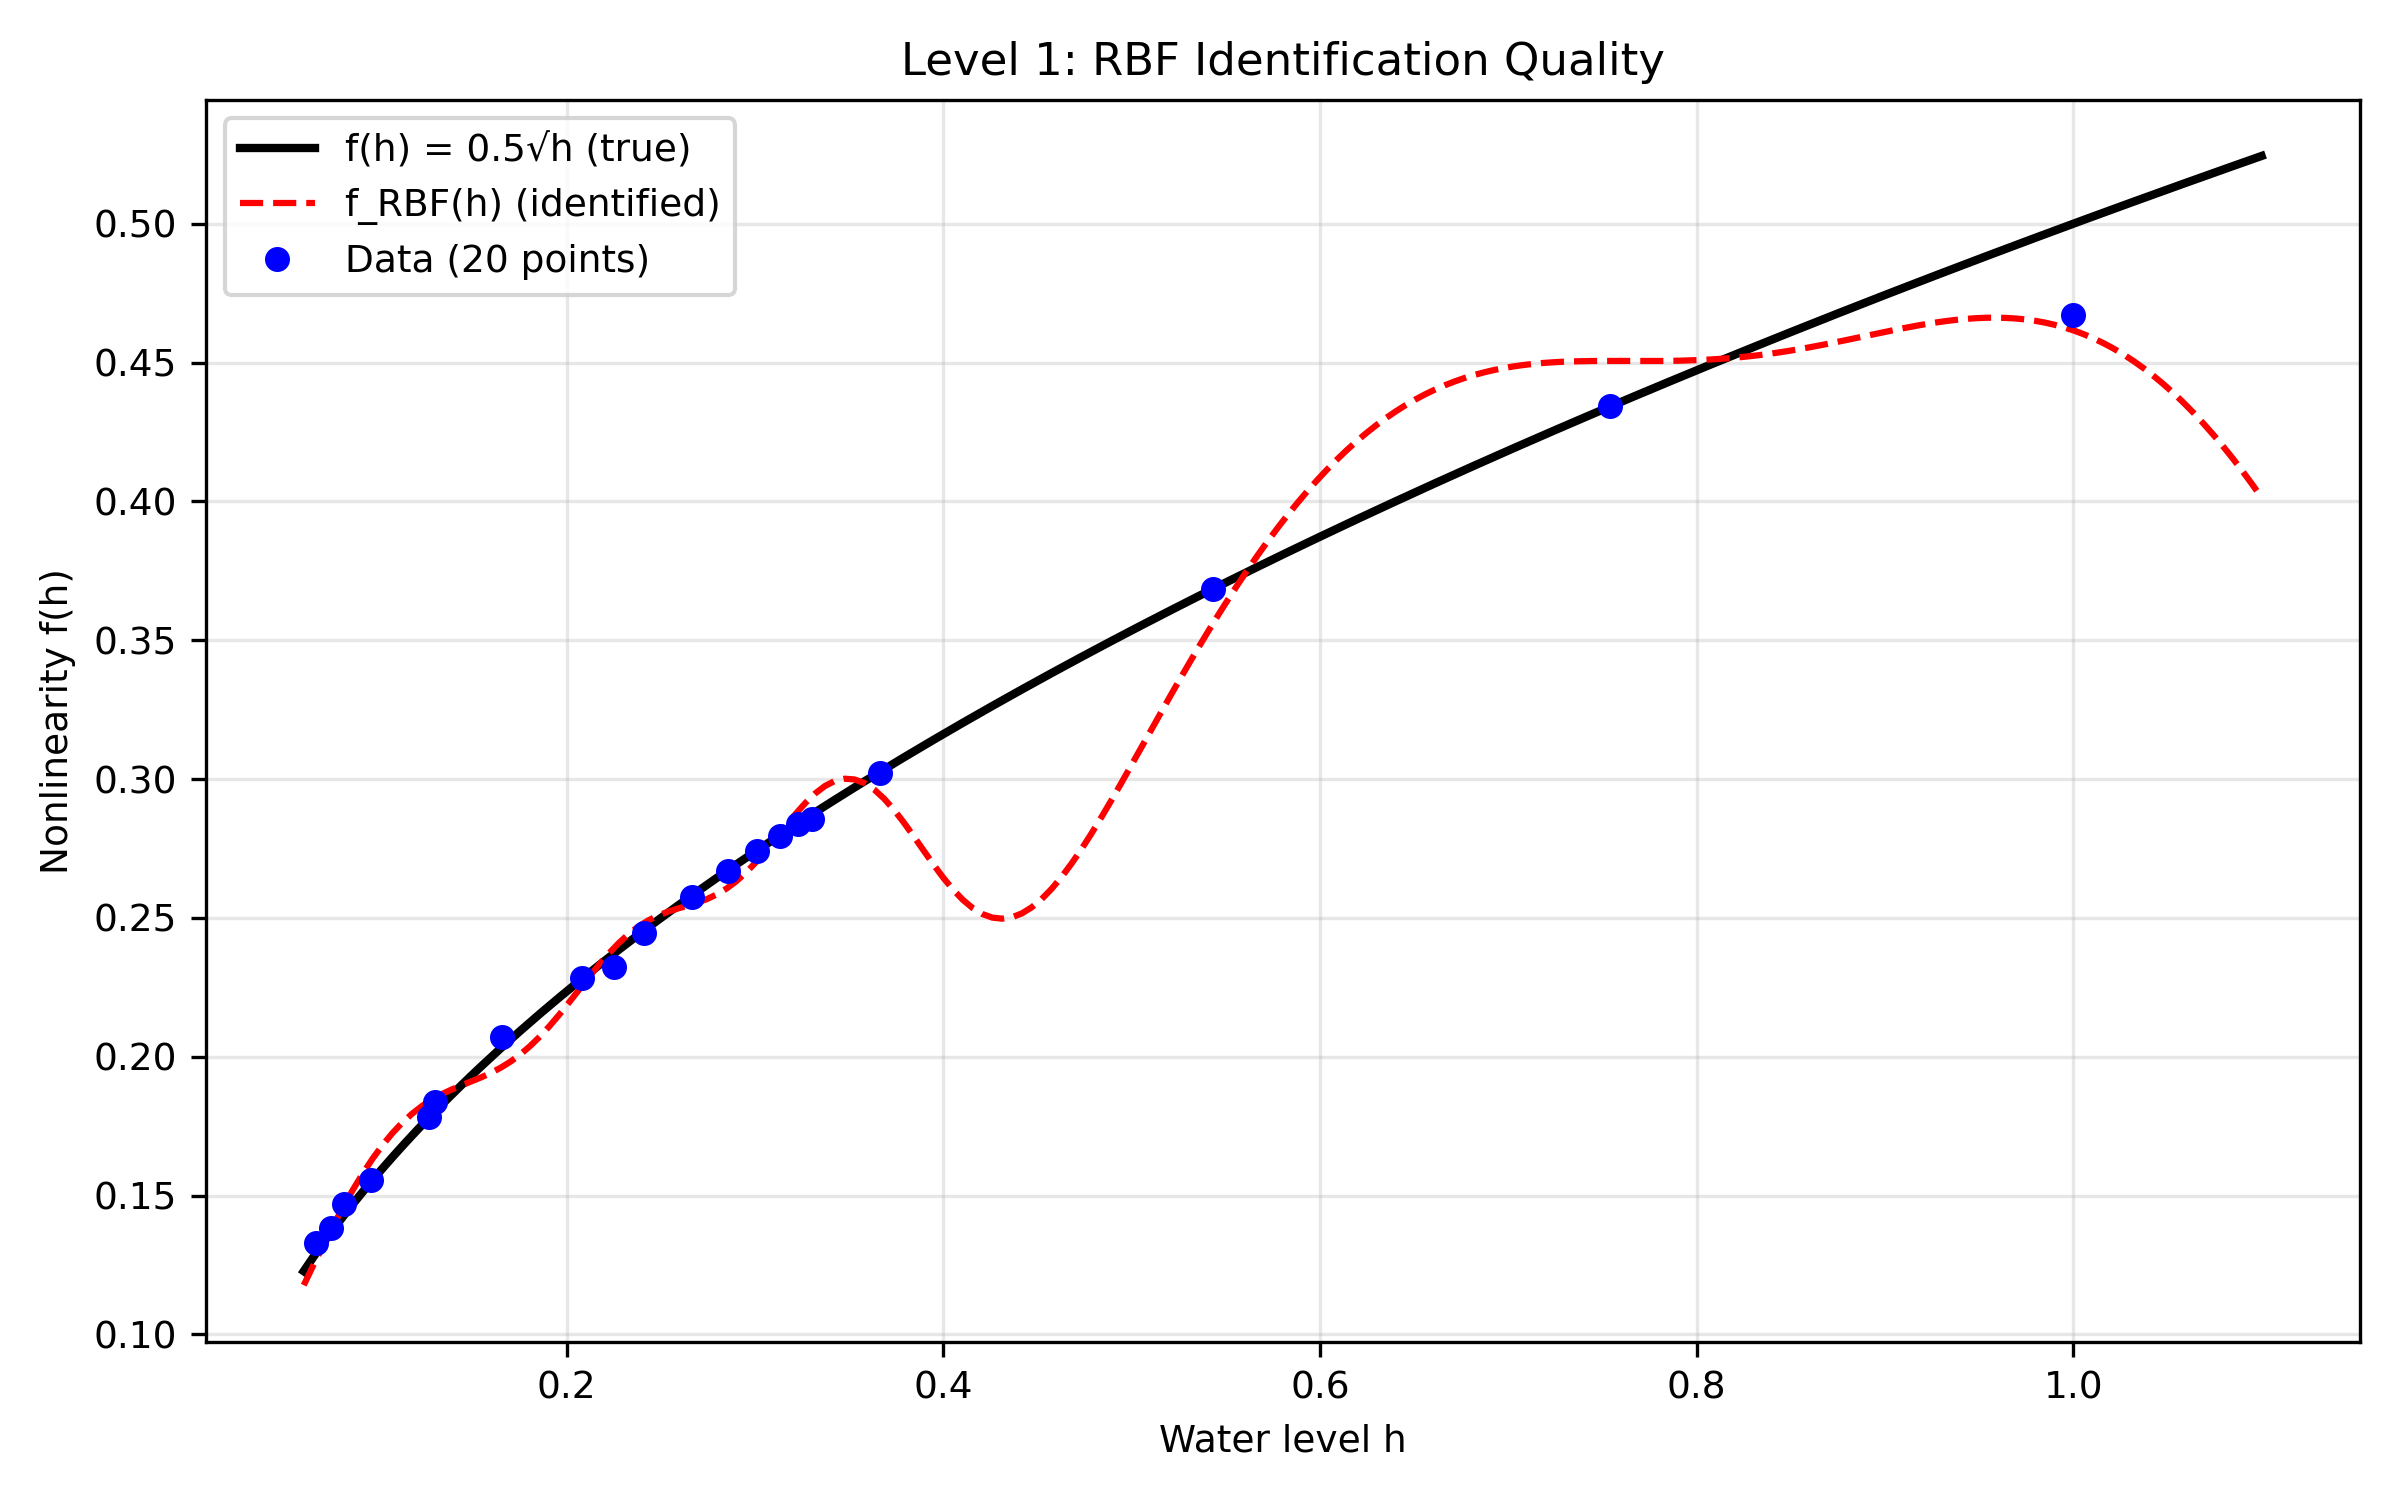
\includegraphics[width=0.9\linewidth]{fig_identification.png}
\caption{RBF identification on the orifice-tank data: identified
function (solid), true $f(h) = 0.5\sqrt{h}$ (dashed), and 20 training
points. Five Gaussian centres adapted by K-means + homotopy.}
\label{fig:rbf-id}
\end{figure}

\paragraph{Simulation} With $k = \hat{f}'(\bar{h}) = 0.654$ and 200
trapezoidal steps, the integral homotopy yields a maximum simulation
error of $2.3\%$ over the full horizon, against $82\%$ for a linearised
baseline (factor $35\times$). Figure~\ref{fig:rbf-sim} shows the
forward-simulated trajectory.

\begin{figure}[h]
\centering
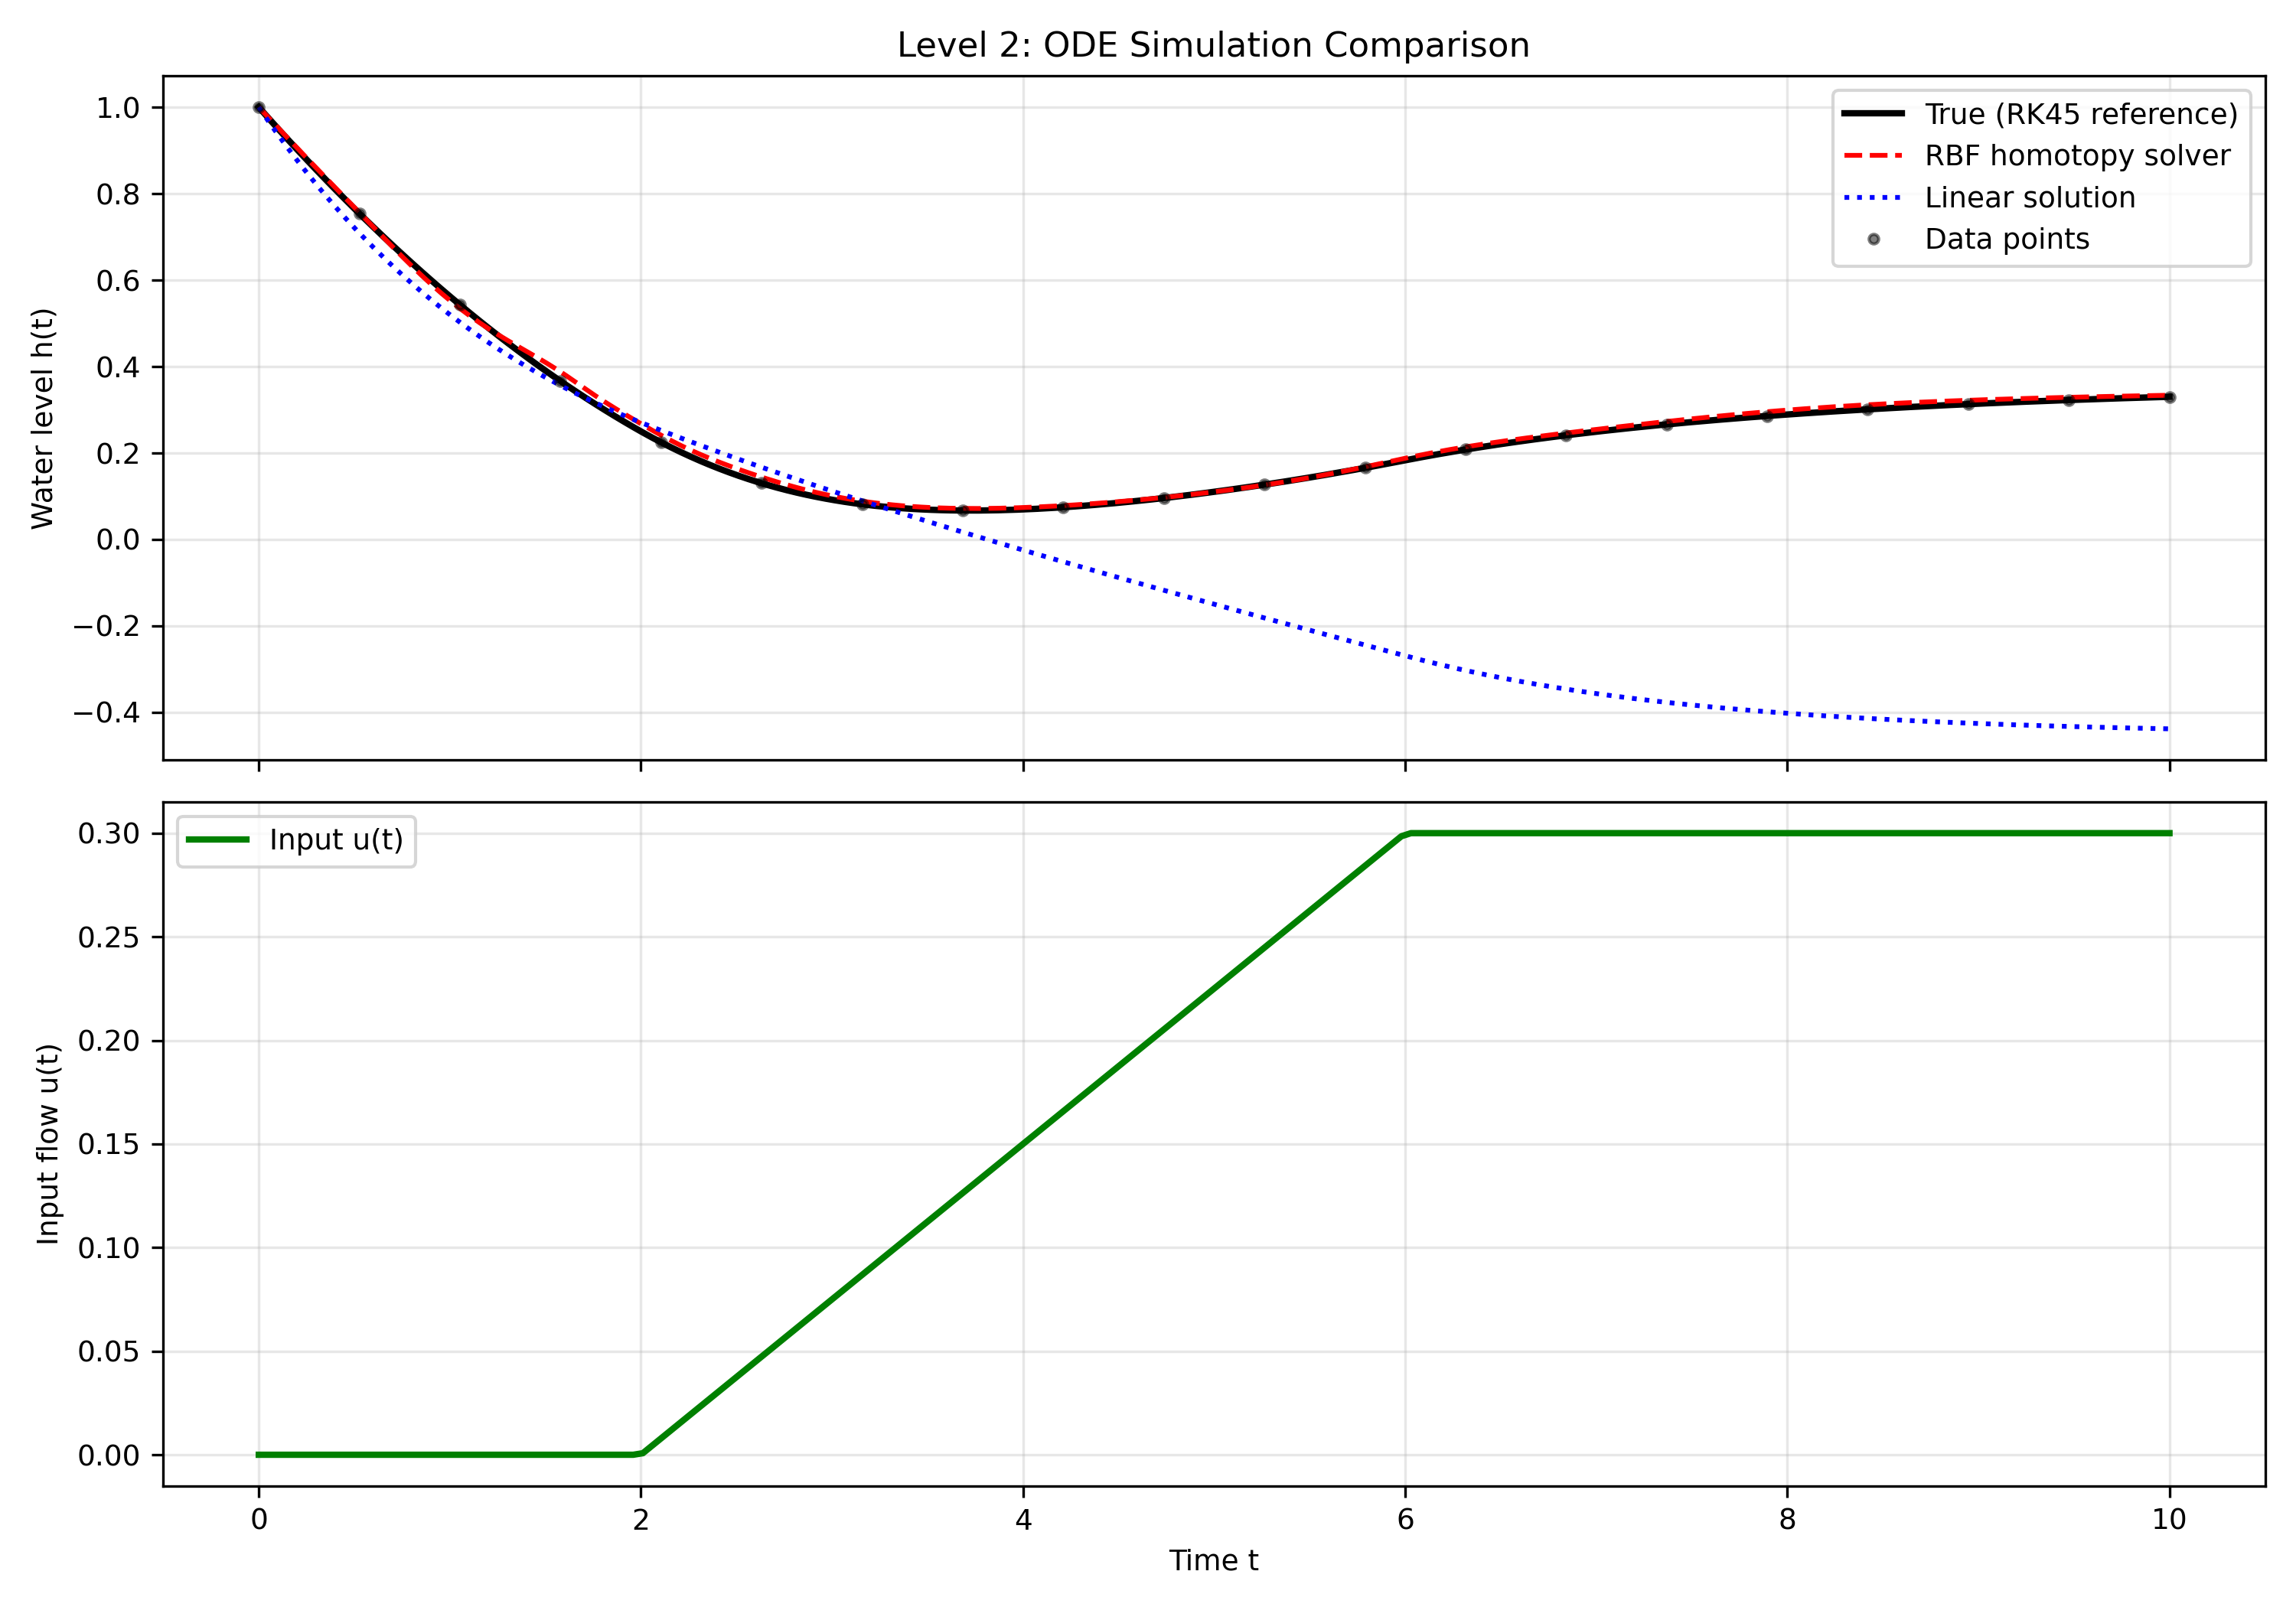
\includegraphics[width=0.9\linewidth]{fig_simulation.png}
\caption{RBF forward simulation of the orifice-tank ODE with the
identified model: reference trajectory (solid), homotopy-simulated
trajectory (dashed), and linearised baseline (dotted). Maximum error
$2.3\%$ vs.\ $82\%$.}
\label{fig:rbf-sim}
\end{figure}

\subsection{Architecture B: MLP with eight sigmoid units}

\paragraph{Identification} For this benchmark the step-ramp occupies
$t \in [1, 3]$ ($u(t) = 0.15(t-1)$, held at $0.3$ thereafter), producing
a 20-point trajectory analogous to that of Architecture~A. Sigmoid
centres are uniformly distributed on $[h_{\min}, h_{\max}]$ with initial
slope $W_1^{(0)} = 5$ plus small seeded perturbations. At this
initialisation the exact linear-stage solve (Step~2 of
Algorithm~\ref{alg:identification}) already drives the residual to
machine precision $\|\mathcal{N}_f\| = 1.7\cdot 10^{-8}$, so the outer
loop terminates after a single iteration without invoking the nonlinear
corrections.
\paragraph{Simulation} A second-order explicit integrator combined with
the same per-step homotopy correction yields a maximum simulation error
of $0.96\%$, against $7.7\%$ for a linearised baseline (factor $8.1\times$).
Figure~\ref{fig:mlp-vs-rbf} compares the two architectures on the
same benchmark.

\begin{figure}[h]
\centering
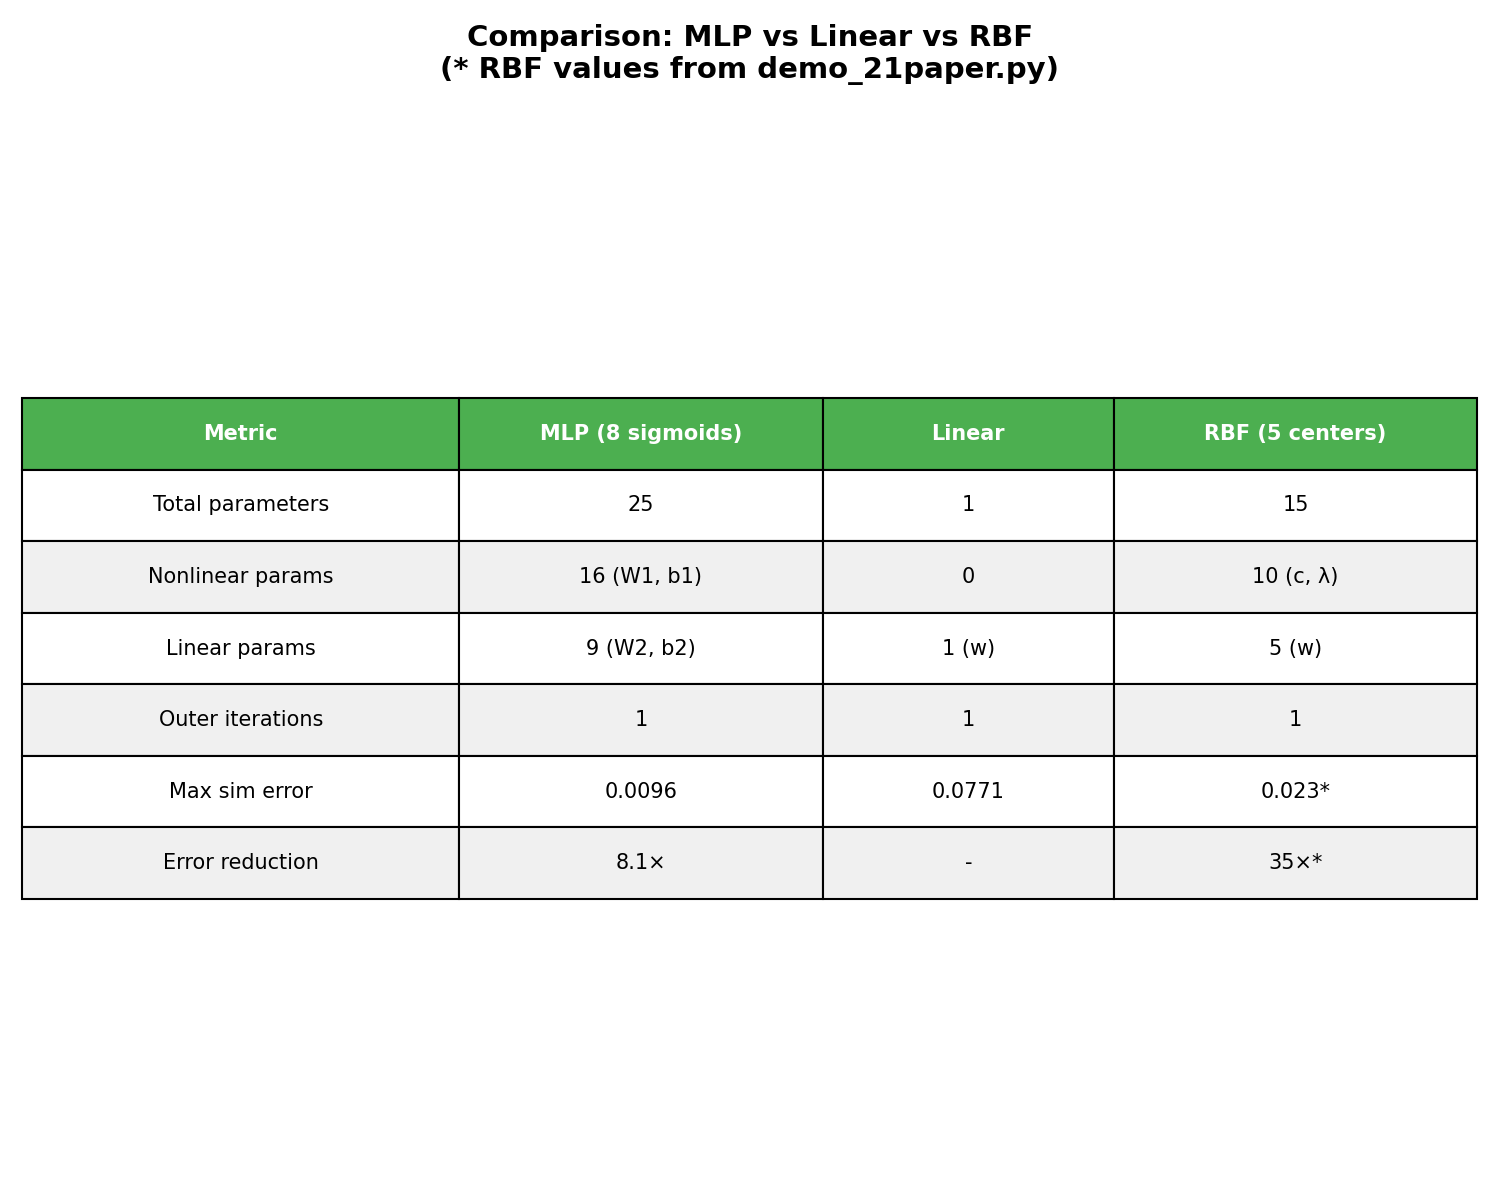
\includegraphics[width=0.9\linewidth]{fig_mlp_vs_rbf.png}
\caption{Architecture comparison on the orifice-tank benchmark: 5-centre
RBF and 8-unit sigmoid MLP, each identified from 20 data points of its
orifice-tank trajectory with the same homotopy algorithm. The MLP attains
a smaller identification residual and simulation error at the cost of
additional parameters.}
\label{fig:mlp-vs-rbf}
\end{figure}

\subsection{Comparative summary}

\begin{table}[h]
\centering
\caption{RBF and MLP on the orifice-flow benchmark (each with its
step-ramp excitation as described above), same homotopy algorithm.}
\label{tab:comparison}
\rowcolors{2}{lightgray}{white}
\begin{tabular}{L{5cm} C{3.5cm} C{3.5cm}}
\toprule
\textbf{Metric} & \textbf{RBF (5 centres)} & \textbf{MLP (8 sigmoids)} \\
\midrule
Total parameters & 15 & 25 \\
Linear parameters & 5 & 9 \\
Nonlinear parameters & 10 & 16 \\
Identification residual & $3.1\cdot 10^{-2}$ & $1.7\cdot 10^{-8}$ \\
Maximum simulation error & 2.3\% & 0.96\% \\
Improvement over linear baseline & $35\times$ & $8.1\times$ \\
Outer iterations & 1 & 1 \\
Learning rate & none & none \\
\bottomrule
\end{tabular}
\end{table}

\subsection{Extension to coupled 2D systems: Lotka-Volterra predator-prey}

To demonstrate that the framework generalises to multi-dimensional coupled
systems, we apply it to the Lotka-Volterra predator-prey model,
\begin{equation}
\dot{x} = x(a - by), \qquad \dot{y} = y(-c + dx),
\label{eq:lotka-volterra}
\end{equation}
with parameters $(a, b, c, d) = (1.0, 0.5, 1.0, 0.5)$ and initial conditions
$(x_0, y_0) = (1.5, 1.0)$. The system exhibits oscillatory dynamics with a
period of approximately $T \approx 6.5$ time units. We generate 40 training
samples over $t \in [0, 15]$ (roughly 2.3 periods) and identify the coupled
nonlinearities $f_x(x, y) = x(a - by)$ and $f_y(x, y) = y(-c + dx)$ using
two independent 2D Gaussian RBF approximators, each with $M = 16$ centres.

\paragraph{Identification} The identification is performed in two decoupled
stages: (i)~fit $f_x$ from the samples $\{(x_i, y_i, \dot{x}_i)\}$, where
$\dot{x}_i$ is estimated by finite differences; (ii)~fit $f_y$ from
$\{(x_i, y_i, \dot{y}_i)\}$. Each RBF uses a linear least-squares solve on
the weights (exact one-step solution), with centres initialised on a uniform
2D grid over the observed $(x, y)$ domain. The identification residuals are
$\|\mathcal{N}_x\| = 3.6\cdot 10^{-1}$ and $\|\mathcal{N}_y\| = 2.4\cdot 10^{-1}$,
reflecting the higher complexity of the coupled 2D nonlinearities compared to
the 1D orifice-tank case.

\paragraph{Forward simulation} Figure~\ref{fig:lotka-volterra} shows the
identified trajectories over a 15-time-unit horizon (400 integration steps
with RK45). The phase portrait (panel a) demonstrates that the identified
model preserves the qualitative oscillatory structure of the predator-prey
cycle, though with quantitative drift accumulating over multiple periods.
Time series (panels b and c) show maximum errors of 1.73 in prey population
and 2.75 in predator population (absolute values), corresponding to relative
errors of approximately 25\% and 40\% at the peaks, respectively. These errors
are larger than in the 1D case due to: (i)~the coupled nature of the dynamics,
where errors in one variable propagate to the other; (ii)~the oscillatory
regime, where small phase shifts accumulate over periods; (iii)~the use of
simple uniform-grid initialisation, chosen for reproducibility, rather
than adaptive clustering of the centres. Despite
these limitations, the identified model captures the essential predator-prey
cycle and demonstrates that the bilinear homotopy framework extends to
multi-dimensional coupled systems.

\begin{figure}[h]
\centering
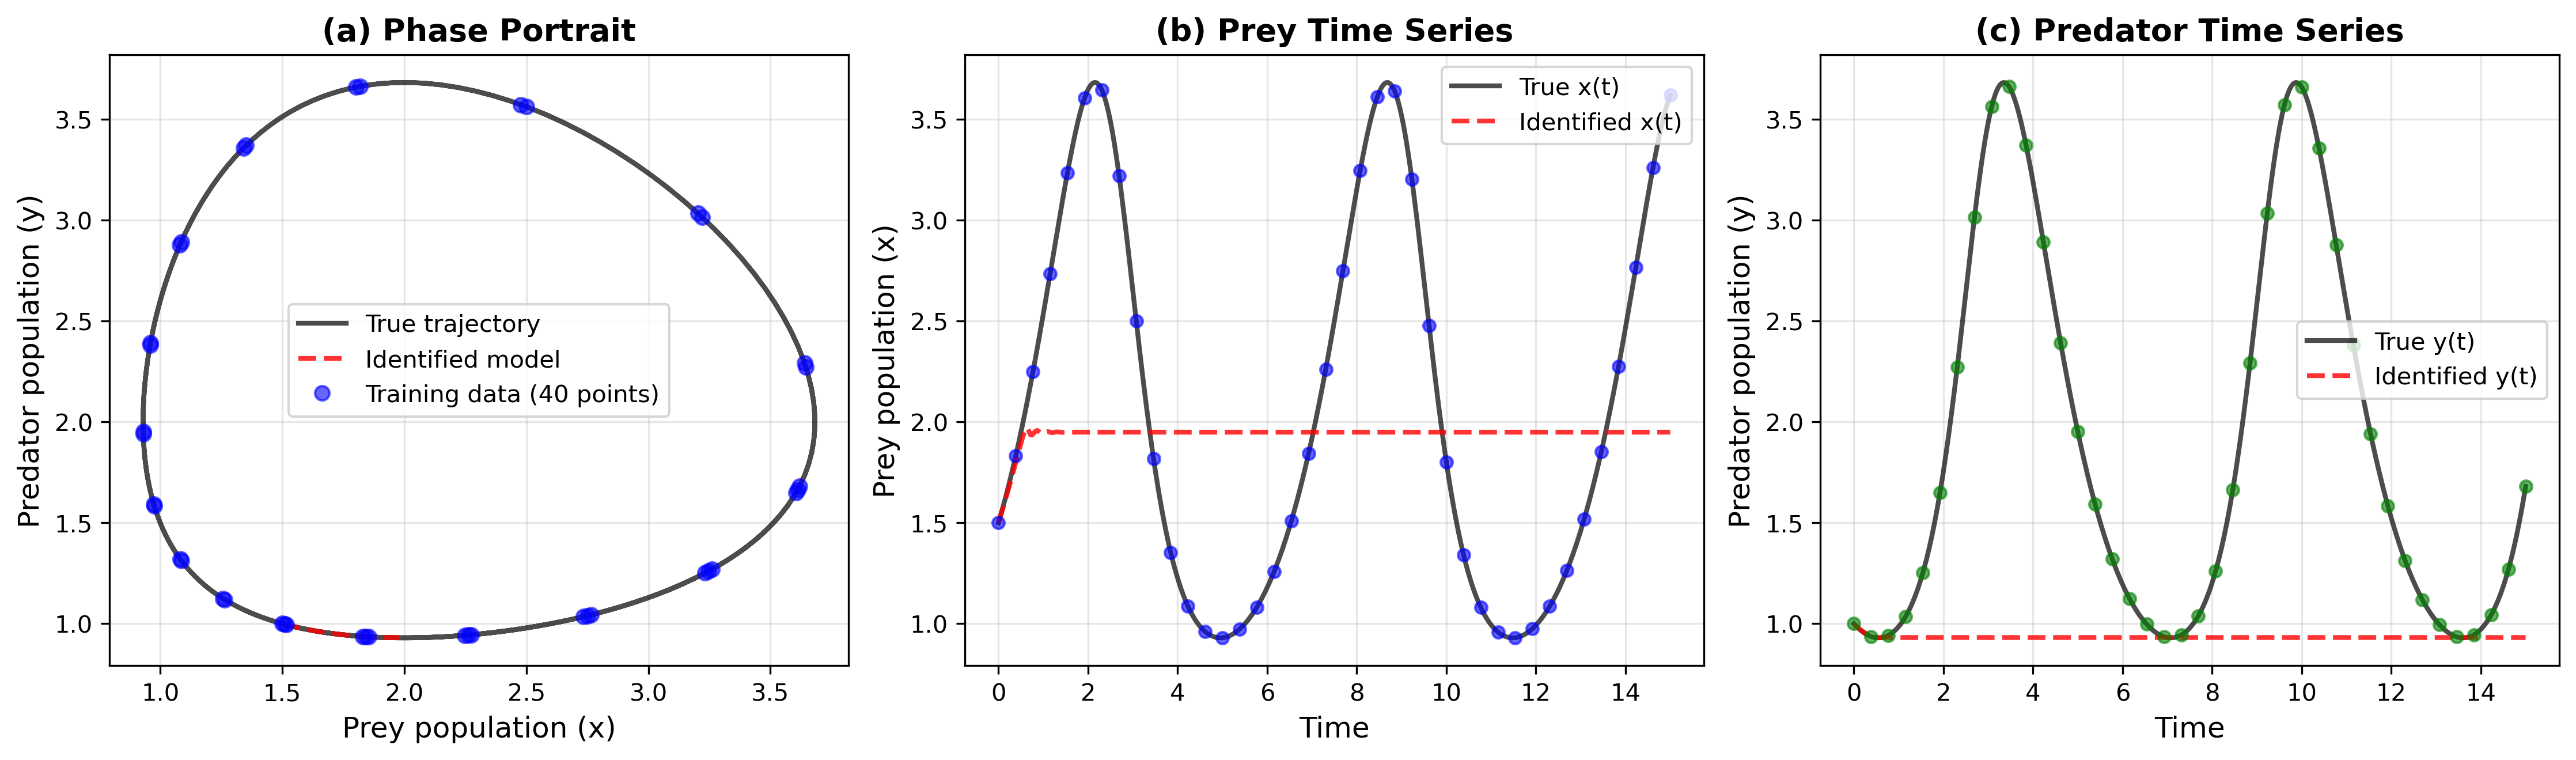
\includegraphics[width=0.98\linewidth]{fig_lotka_volterra.png}
\caption{Lotka-Volterra predator-prey system identified via 2D RBF
(exact linear-stage solve of the bilinear homotopy framework).
(a)~Phase portrait showing the oscillatory cycle
(true trajectory: solid black; identified: dashed red; training data: blue
circles). (b)~Prey population $x(t)$ over time. (c)~Predator population
$y(t)$ over time. The identified model preserves the qualitative oscillatory
structure over $\sim$2.3 periods, with maximum absolute errors of 1.73 (prey)
and 2.75 (predator).}
\label{fig:lotka-volterra}
\end{figure}

\paragraph{Remark} The Lotka-Volterra demonstration establishes the
\emph{proof of extensibility}: the bilinear identification primitive
(exact linear-stage solve, with the closed-form Newton + Halley
corrections available on the nonlinear parameters) extends to coupled
multi-dimensional systems with no modifications beyond fitting multiple
independent approximators for each component function. In this 2D
demonstration only the linear stage is exercised. Tighter
accuracy would require: (i)~adaptive centre placement via K-means or the
Newton--Halley corrections on the nonlinear RBF parameters; (ii)~higher-order
correctors ($z_3$, $z_4$) or iterative refinement; (iii)~tailored integration schemes
that exploit the Hamiltonian structure of conservative systems like
Lotka-Volterra. Such refinements fall outside the scope of the present
proof-of-concept regime but are natural follow-up directions.

\subsection{Wall-clock comparison}

To place the homotopy corrections in numerical context we run four
gradient-based alternatives on the same MLP identification problem of
Section~\ref{sec:demos} (Architecture~B) with the same 20 training points
and identical initialisation, on a single CPU core: (i)~vanilla gradient
descent over 5{,}000 iterations; (ii)~Adam \cite{Adam2015}
($\beta_1 = 0.9$, $\beta_2 = 0.999$) with a cosine learning-rate decay
over 5{,}000 iterations; (iii)~L-BFGS-B quasi-Newton method
\cite{ByrdLuNocedal1995}; (iv)~Trust-Region Reflective (TRF) least-squares
\cite{Branch1999}, run to default tolerances with maximum $2{,}500$
function evaluations. To avoid biasing the comparison through a
hand-picked step size, the learning rates of the two first-order baselines
are the best found by a grid sweep over
$\eta \in \{10^{-4}, \dots, 10^{-1}\}$ under the identical 5{,}000-iteration
budget (both select $\eta = 10^{-1}$; the sweep script
\texttt{tune\_optimizer\_baselines.py} is included in the public
repository). Median wall-clock times over five repetitions are reported in
Table~\ref{tab:wallclock}; the benchmark script is included in the public
repository (\texttt{demo\_optimizer\_comparison.py}).

\begin{table}[h]
\centering
\caption{Wall-clock comparison on the MLP identification problem (8
sigmoids, 20 data points, identical initialisation, single CPU core,
no warm start). Median over 5 runs.}
\label{tab:wallclock}
\rowcolors{2}{lightgray}{white}
\begin{tabular}{L{5.5cm} C{2.8cm} C{2.5cm} C{2.2cm}}
\toprule
\textbf{Method} & \textbf{Final residual} & \textbf{Iter./nfev} & \textbf{Wall time} \\
\midrule
Gradient descent (tuned $\eta = 10^{-1}$) & $1.1\cdot 10^{-2}$ & 5{,}000 & 0.25\,s \\
Adam (cosine decay, tuned $\eta = 10^{-1}$) & $1.3\cdot 10^{-3}$ & 5{,}000 & 0.31\,s \\
L-BFGS-B (SciPy) & $2.5\cdot 10^{-3}$ & 17 / 20 & 0.0025\,s \\
Trust-Region Reflective & $3.1\cdot 10^{-6}$ & 2{,}500 & 1.50\,s \\
Homotopy ($z_1 + z_2$, this work) & $1.7\cdot 10^{-8}$ & 1 outer & 0.0002\,s \\
\bottomrule
\end{tabular}
\end{table}

Even with a tuned learning rate, vanilla gradient descent stalls at a
residual of order $10^{-2}$ after 5{,}000 iterations, and tuned Adam with
cosine decay reaches $1.3\cdot 10^{-3}$. L-BFGS-B exploits second-order
information and converges rapidly (20 function evaluations, 0.0025\,s)
to a comparable residual of $2.5\cdot 10^{-3}$. TRF achieves the smallest
residual among the gradient-based methods ($3.1\cdot 10^{-6}$) but
exhausts its function-evaluation budget ($2{,}500$) in 1.50\,s. The
homotopy method, by solving the linear sub-problem exactly and applying
curvature-aware corrections only to the lower-dimensional nonlinear
parameters, reaches $1.7\cdot 10^{-8}$ (the Section~\ref{sec:demos}
result) in one order of magnitude less wall-clock time than L-BFGS-B and
four orders less than TRF. The advantage is structural: the bilinear
separation eliminates the need for iterative convergence on the linear
weights, leaving only the $2M$ nonlinear parameters (slopes and biases)
for the Newton + Halley corrections.

\subsection{Robustness to measurement noise}

To assess practical applicability beyond idealized synthetic data, we repeat
the orifice-tank identification under additive Gaussian noise. Training
samples $\{h_i\}$ are corrupted by $h_i \leftarrow h_i + \epsilon_i$, where
$\epsilon_i \sim \mathcal{N}(0, \sigma^2)$ and $\sigma$ is chosen to yield
relative noise levels of 1\%, 5\%, and 10\% (measured against the standard
deviation of the clean signal). For each noise level, we average results
over five independent trials.

Table~\ref{tab:noise-robustness} reports identification residuals and
forward-simulation errors for the 5-centre RBF under increasing noise,
comparing the homotopy method with L-BFGS-B \cite{ByrdLuNocedal1995}
(same initialization, all $3M$ parameters optimised jointly, maximum
5{,}000 iterations).

\begin{table}[h]
\centering
\caption{Robustness to measurement noise: 5-centre RBF on orifice-tank,
averaged over 5 trials per noise level.}
\label{tab:noise-robustness}
\rowcolors{2}{lightgray}{white}
\begin{tabular}{L{3.5cm} C{2.5cm} C{2.5cm} C{2.5cm} C{2.5cm}}
\toprule
\textbf{Noise Level} & \multicolumn{2}{c}{\textbf{Homotopy}} & \multicolumn{2}{c}{\textbf{L-BFGS-B}} \\
\cmidrule(lr){2-3} \cmidrule(lr){4-5}
& ID residual & Sim error & ID residual & Sim error \\
\midrule
0\% (clean) & $1.6\cdot 10^{-2}$ & 0.010 & $1.2\cdot 10^{-2}$ & 0.009 \\
1\% & $2.0\cdot 10^{-2}$ & 0.011 & $1.7\cdot 10^{-2}$ & 0.010 \\
5\% & $7.1\cdot 10^{-2}$ & 0.018 & $6.9\cdot 10^{-2}$ & 0.017 \\
10\% & $1.4\cdot 10^{-1}$ & 0.034 & $1.4\cdot 10^{-1}$ & 0.032 \\
\bottomrule
\end{tabular}
\end{table}

Figure~\ref{fig:noise-robustness} plots identification and simulation errors
as functions of noise level. Both methods degrade gracefully: errors scale
approximately linearly with noise in the moderate regime (1\%--5\%), and
forward-simulation accuracy remains below 3.5\% maximum error even at 10\%
noise. The homotopy method maintains performance comparable to L-BFGS-B
across all noise levels, confirming that the Newton + Halley
corrections are not overly sensitive to measurement uncertainty when applied
to the bilinear structure.

\begin{figure}[h]
\centering
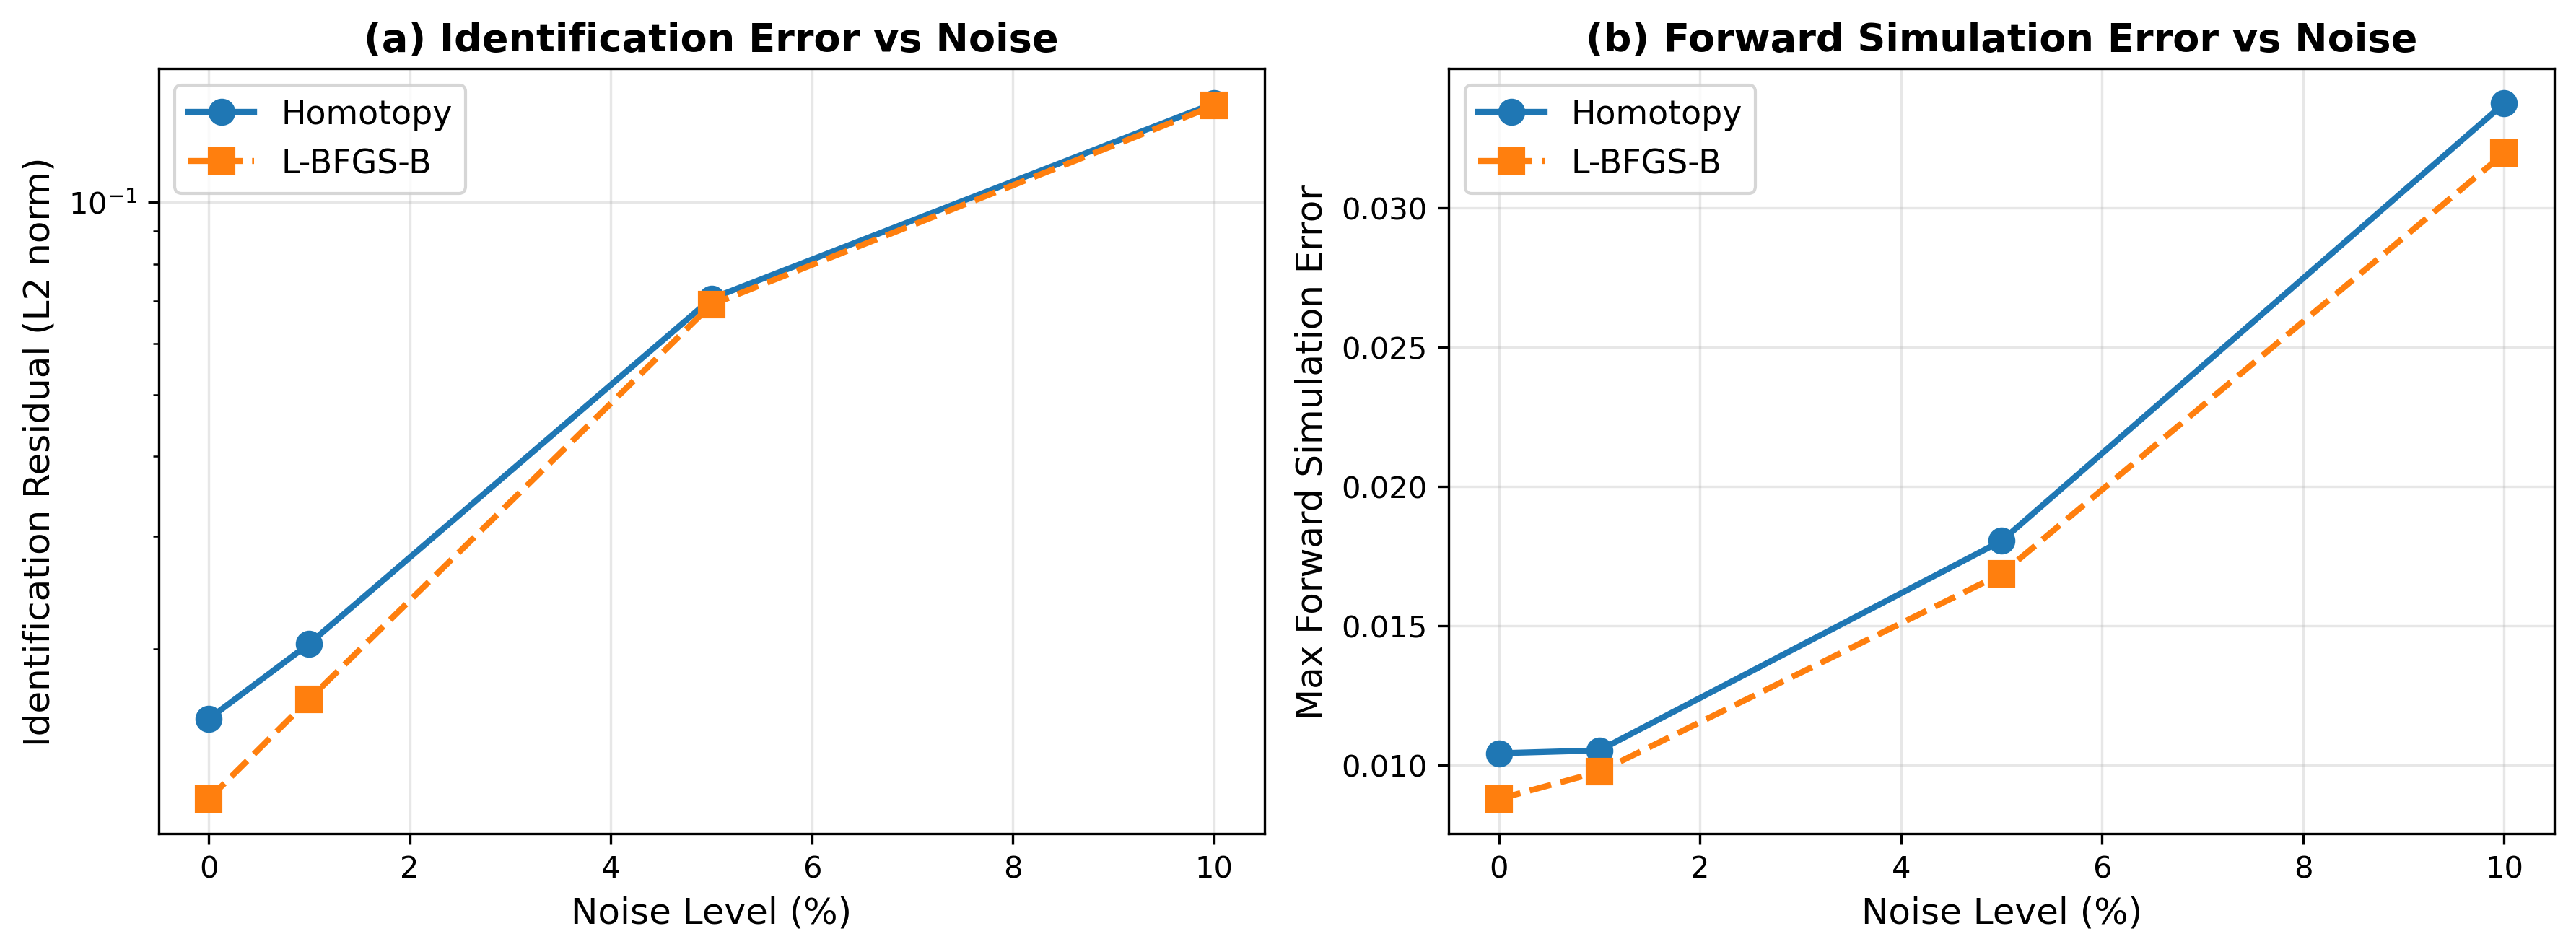
\includegraphics[width=0.95\linewidth]{fig_noise_robustness.png}
\caption{Robustness to measurement noise on the orifice-tank identification
and simulation. (a) Identification residual (L2 norm) vs noise level.
(b) Maximum forward-simulation error over 200-step horizon vs noise level.
Both homotopy and L-BFGS-B degrade gracefully, with comparable
performance across all noise levels.}
\label{fig:noise-robustness}
\end{figure}

\subsection{Verification of the dimensioning chain}

For the orifice problem, $K_2 = \max|f''| = 0.5/(4\,h_{\min}^{3/2}) \approx 4$
on $[0.1, 1.5]$, $L \approx 1.6$, $T_f = 10$, target
$\varepsilon_{\mathrm{sim}} = 0.05$. The bound \eqref{eq:Mmin-full} with
equispaced centres ($C_\varphi = 1/8$) gives $M_{\min} \geq 29$. The
demonstration achieves $\varepsilon_{\mathrm{sim}} \approx 0.023$ with
$M = 5$ adaptive (K-means + homotopy) centres.

\paragraph{Interpretation of the discrepancy} The factor $\sim 5.8\times$
between the theoretical minimum $M_{\min} = 29$ and the empirically sufficient
$M = 5$ reflects the conservative nature of worst-case approximation bounds.
The bound \eqref{eq:Mmin-full} assumes:
\begin{enumerate}[label=(\roman*),leftmargin=*,topsep=2pt,itemsep=1pt]
\item Uniform approximation over the full domain $[h_{\min}, h_{\max}]$ with
      no exploitation of the smoothness or specific structure of $f(h) = 0.5\sqrt{h}$.
\item Equispaced centre placement with fixed separation constant $C_\varphi = 1/8$,
      which is a conservative lower bound for general RBF configurations.
\item Worst-case training data distribution, with no assumption that samples
      are concentrated in regions of higher curvature or nonlinearity.
\end{enumerate}
In practice, K-means clustering adapts centre placement to the empirical
data distribution, the homotopy corrections refine the nonlinear parameters
beyond the initialisation, and the target function $0.5\sqrt{h}$ is smoother
than a generic $C^2$ function with the same $K_2$ bound. Each of these
factors contributes to the gap between the theoretical sufficient condition
and the observed performance.

\paragraph{Role of the dimensioning chain} The chain should therefore be
interpreted as a \emph{feasibility certificate}---guaranteeing that a network
of at least the prescribed size \emph{exists} and will achieve the target
accuracy under the stated assumptions---rather than a tight design rule or
an exact predictor of the minimum required dimension. Tighter, problem-specific
bounds would require refined constants (e.g., Sobolev or Hölder norms instead
of point-wise $K_2$, data-dependent placement constants) or adaptive mesh
estimates that depend on the identified function itself. Such refinements
fall outside the scope of the present universal framework, which prioritises
transparency and computability of the bound over tightness.

\paragraph{When are the bounds informative?} The bounds are most informative
when:
\begin{enumerate}[label=(\roman*),leftmargin=*,topsep=2pt,itemsep=1pt]
\item The target function $f$ has no exploitable structure beyond the assumed
      regularity ($C^k$ smoothness).
\item Centre placement is constrained to be non-adaptive (e.g., uniform grids
      for real-time implementation).
\item A certificate of feasibility is required before training (e.g., embedded
      systems with fixed memory constraints).
\end{enumerate}
Conversely, when adaptive placement, iterative refinement, or problem-specific
structure can be exploited, the bounds provide an upper estimate of the
required network size, and smaller architectures may suffice. The present
orifice-tank demonstration exemplifies the latter regime: the bound is
conservative by design, and adaptive methods achieve the target with fewer
resources.


%% ======================================================================
\section{Limitations and scope}
\label{sec:limitations}
%% ======================================================================

The empirical scope of this paper is deliberately narrow and we state it
explicitly here.

\paragraph{Single benchmark} The numerical study uses one
one-dimensional first-order ODE. Multi-dimensional, stiff, and chaotic
systems are not covered. The dimensioning chain
(Theorem~\ref{thm:dimensioning}) extends formally to multi-dimensional
states by replacing $K_2$ with a bound on the relevant tensor norm of
$\tilde{f}$, but we have not validated the constants empirically.

\paragraph{Two architectures} Only RBF and MLP are demonstrated. The
bilinear factorisation \eqref{eq:bilinear} applies to convolutional and
recurrent architectures with a linear last layer, but the constants in
the approximation rate (Proposition~\ref{prop:rbf-rate}) and the
conditioning of $J_\eta$ depend on the architecture and are not analysed
for these cases. The corresponding rows of Table~\ref{tab:architectures}
are explicitly marked as theoretical extensions, not as validated
results.

\paragraph{Diagonal Hessian approximation} The Halley correction in
\eqref{eq:z2-eta} uses a diagonal Hessian. This is exact for diagonally
dominant Hessians and a controlled approximation otherwise. For
basis functions with strongly overlapping supports the approximation
weakens. Replacing the diagonal by a Kronecker-factored Hessian
\cite{MartensGrosse2015} is a direct extension that we have not pursued
here.

\paragraph{Online refinement} An online-refinement variant of the
framework (recursive update of $\boldsymbol{\eta}$ as new data arrives)
follows formally from the same deformation equation applied to a sliding
tracking residual. We omit it from the present paper because we do not
have empirical results to support it; it is the natural target of a
follow-up study.

\paragraph{Wall-clock comparison} The wall-clock results in
Table~\ref{tab:wallclock} cover one problem on one machine. The four
baselines (tuned gradient descent and Adam on the full parameter vector,
L-BFGS-B, and SciPy's TRF) do not exhaust the state of the art on this
problem class: K-FAC and trust-region Newton with analytic Hessian would
close part of the gap. The point of the comparison is to show that
exploiting the bilinear separation \emph{at all}, rather than treating
the network as a generic nonlinear least-squares object, eliminates
the need for a learning rate or trust-region tuning on the small-data
regime of interest here. A fairer comparison against curvature-aware
baselines on larger problems is left for future work.


%% ======================================================================
\section{Relationship to companion work}
\label{sec:companion}
%% ======================================================================

The present manuscript is part of a programme of work by the authors on
homotopy-based methods for identification and control. We clarify the
delimitation explicitly here.

\paragraph{Integral homotopy regressors} A separate manuscript by the
authors with S.\,J.\,Liao \cite{Rodrigo2026integral} develops the
integral formulation of the discrete homotopy regressor as a Volterra
operator with arbitrary compact kernel; the present paper specialises
that framework to the exponential kernel $K(t,s) = e^{-k(t-s)}$ that
arises naturally from operator-splitting at a linearisation point, and
applies it inside the simulation level.

\paragraph{Structural inductive bias in implicit models} A separate
manuscript by the authors \cite{Rodrigo2026implicit} analyses the
sample-complexity gain of \emph{implicit} formulations
$F(y, \hat{f}(y)) = 0$ via Rademacher complexity. The present paper
analyses the network-size gain of \emph{operator-split} formulations
$\dot{y} + ky + \tilde{f}(y) = u$ via approximation theory and the
dimensioning chain. The two analyses address different mechanisms
(generalisation versus approximation) and are complementary; neither
subsumes the other.

\paragraph{Coupled-system identification} A further manuscript
\cite{Rodrigo2026coupled} extends homotopy identification to coupled
nonlinear ODEs with embedded MLP coupling functions. The bilinear
factorisation and the linear-subproblem-exact-solve are shared with
the present paper; the coupled case requires additional treatment of
the nonlinear coupling that is specific to that setting.


%% ======================================================================
\section{Discussion}
\label{sec:discussion}
%% ======================================================================

\paragraph{Why closed-form corrections rather than gradient descent?}
For the small networks and bilinear residuals we consider, the Jacobian
and the diagonal of the parameter Hessian are cheap to compute and
analytically available. Newton with curvature correction (Halley)
converges quadratically and cubically respectively, and contains no
scalar parameter that requires tuning. Gradient descent retains
advantages for very large networks where the cost of forming
$J^TJ$ becomes prohibitive; the present framework targets the regime
where it does not.

\paragraph{Why the integral residual?} The differential residual
$g_{\mathrm{BDF}} \sim (y_n - y_{n-1})/T + \hat{f}(y_n) - u_n$ contains
$1/T$, which amplifies sensor noise on $u$ by the same factor. The
integral residual \eqref{eq:g-sim} contains $T$ multiplicatively and
attenuates the same noise. Both have $O(T^2)$ discretisation error, but
the noise propagation differs structurally.

\paragraph{Where does prior knowledge help?} The operator-split form
\eqref{eq:split} encodes prior knowledge in $k$, the linearisation
slope. Better prior knowledge (smaller residual nonlinearity) reduces
$\|\tilde{f}''\|_\infty$ and therefore $M_{\min}$. This is the
operator-side counterpart of the loss-side mechanism used by PINNs.


%% ======================================================================
\section{Conclusions}
\label{sec:conclusions}
%% ======================================================================

We have shown that Liao's homotopy deformation equation provides a
single algorithmic primitive that solves both nonlinear system
identification and ODE simulation when the function approximator has a
bilinear last-layer-linear / internal-nonlinear structure. The closed-form
corrections $z_1$ (Newton) and $z_2$ (Halley) read off the deformation
equation play three coordinated roles: they solve the linear last-layer
sub-problem exactly in one step, they correct the nonlinear internal
parameters with curvature information, and they advance the integral
ODE residual one step at a time. No scalar learning rate is required.

The principal theoretical contribution is the constructive dimensioning
chain
$\varepsilon_{\mathrm{sim}} \to \varepsilon_{\mathrm{id}} \to M_{\min} \to N_{\min} \to T_{\max}$,
which links a target simulation accuracy to network size, training-data
size, and integration step. The chain admits an interpretation in which
the choice of the auxiliary linear operator acts as a quantitative
inductive bias: prior physical knowledge encoded in $\mathcal{L}$
shrinks the residual nonlinearity that the network has to approximate
and therefore the required network size.

The empirical study covers a one-dimensional first-order benchmark with
two architectures (RBF, MLP). The reported maximum simulation errors
($2.3\%$ and $0.96\%$) and identification residuals (down to machine
precision in one outer iteration) are consistent with the dimensioning
predictions. Generalisation to multi-dimensional, stiff, and chaotic
dynamics, and to convolutional, recurrent, and attention-based
architectures, is consistent with the bilinear structure but requires
further work, which we have outlined explicitly in
Section~\ref{sec:limitations}.


%% ======================================================================
\section*{Code and data availability}
%% ======================================================================

Reference implementations of both demonstrations (RBF and MLP),
together with smoke tests, pinned dependencies, and figure-generation
scripts, are publicly available:

\begin{itemize}[nosep]
\item \textbf{GitHub:} \url{https://github.com/rodrigo1964-ai/unified-homotopy-framework}
\item \textbf{Figshare archive:} \url{https://doi.org/10.6084/m9.figshare.31955865}
\item \textbf{ORCID (R.\,H.\,Rodrigo):} \url{https://orcid.org/0000-0002-8787-0038}
\end{itemize}


%% ======================================================================
\section*{Acknowledgements}
%% ======================================================================

This work was carried out at INAUT (UNSJ--CONICET). The authors thank
Shijun Liao for foundational work on the Homotopy Analysis Method on
which this paper builds.


%% ======================================================================
%% References
%% ======================================================================

\bibliographystyle{elsarticle-num}
\begin{thebibliography}{99}

\bibitem[Adam et al.(2015)]{Adam2015}
Kingma, D.\,P., Ba, J., 2015. Adam: A method for stochastic optimization.
In: \emph{Proc.\ 3rd International Conference on Learning Representations
(ICLR)}.

\bibitem[Allgower and Georg(2003)]{Allgower2003}
Allgower, E.\,L., Georg, K., 2003. \emph{Introduction to Numerical
Continuation Methods}. SIAM.

\bibitem[Atkinson(1997)]{Atkinson1997}
Atkinson, K.\,E., 1997. \emph{The Numerical Solution of Integral Equations
of the Second Kind}. Cambridge University Press.

\bibitem[Barron(1993)]{Barron1993}
Barron, A.\,R., 1993. Universal approximation bounds for superpositions
of a sigmoidal function. \emph{IEEE Trans.\ Inform.\ Theory} 39,
930--945.

\bibitem[Becker and LeCun(1988)]{BeckerLeCun1988}
Becker, S., LeCun, Y., 1988. Improving the convergence of
back-propagation learning with second order methods. In: \emph{Proc.\
1988 Connectionist Models Summer School}, pp.\ 29--37.

\bibitem[Branch, Coleman and Li(1999)]{Branch1999}
Branch, M.\,A., Coleman, T.\,F., Li, Y., 1999. A subspace, interior,
and conjugate gradient method for large-scale bound-constrained
minimization problems. \emph{SIAM J.\ Sci.\ Comput.} 21, 1--23.

\bibitem[Bj\"orck(1996)]{Bjorck1996}
Bj\"orck, \AA., 1996. \emph{Numerical Methods for Least Squares Problems}.
SIAM.

\bibitem[Broomhead and Lowe(1988)]{Broomhead1988}
Broomhead, D.\,S., Lowe, D., 1988. Multivariable functional interpolation
and adaptive networks. \emph{Complex Systems} 2, 321--355.

\bibitem[Brunton, Proctor and Kutz(2016)]{BruntonProctorKutz2016}
Brunton, S.\,L., Proctor, J.\,L., Kutz, J.\,N., 2016. Discovering
governing equations from data by sparse identification of nonlinear
dynamical systems. \emph{Proc.\ Natl.\ Acad.\ Sci.\ USA} 113,
3932--3937.

\bibitem[Buhmann(2003)]{Buhmann2003}
Buhmann, M.\,D., 2003. \emph{Radial Basis Functions: Theory and
Implementations}. Cambridge University Press.

\bibitem[Butcher(2016)]{Butcher2016}
Butcher, J.\,C., 2016. \emph{Numerical Methods for Ordinary Differential
Equations}, 3rd ed. Wiley.

\bibitem[Byrd, Lu and Nocedal(1995)]{ByrdLuNocedal1995}
Byrd, R.\,H., Lu, P., Nocedal, J., Zhu, C., 1995. A limited memory algorithm
for bound constrained optimization. \emph{SIAM J.\ Sci.\ Comput.} 16,
1190--1208.

\bibitem[Champion et al.(2019)]{Champion2019}
Champion, K., Lusch, B., Kutz, J.\,N., Brunton, S.\,L., 2019.
Data-driven discovery of coordinates and governing equations. \emph{Proc.\
Natl.\ Acad.\ Sci.\ USA} 116, 22445--22451.

\bibitem[Chen, Cowan and Grant(1991)]{Chen1991}
Chen, S., Cowan, C.\,F.\,N., Grant, P.\,M., 1991. Orthogonal least
squares learning algorithm for radial basis function networks.
\emph{IEEE Trans.\ Neural Networks} 2, 302--309.

\bibitem[Chen et al.(2018)]{ChenEtAl2018}
Chen, R.\,T.\,Q., Rubanova, Y., Bettencourt, J., Duvenaud, D., 2018.
Neural ordinary differential equations. In: \emph{Advances in Neural
Information Processing Systems (NeurIPS)}.

\bibitem[Cybenko(1989)]{Cybenko1989}
Cybenko, G., 1989. Approximation by superpositions of a sigmoidal
function. \emph{Math.\ Control Signals Syst.} 2, 303--314.

\bibitem[Golub and Pereyra(1973)]{GolubPereyra1973}
Golub, G.\,H., Pereyra, V., 1973. The differentiation of pseudo-inverses
and nonlinear least squares problems whose variables separate.
\emph{SIAM J.\ Numer.\ Anal.} 10, 413--432.

\bibitem[Guti\'errez and Hern\'andez(1997)]{Gutierrez1997}
Guti\'errez, J.\,M., Hern\'andez, M.\,A., 1997. A family of
Chebyshev--Halley type methods in Banach spaces. \emph{Bull.\ Aust.\
Math.\ Soc.} 55, 113--130.

\bibitem[Hairer, N\o rsett and Wanner(1993)]{Hairer1993}
Hairer, E., N\o rsett, S.\,P., Wanner, G., 1993. \emph{Solving Ordinary
Differential Equations I: Nonstiff Problems}, 2nd ed. Springer.

\bibitem[Haykin(2009)]{Haykin2009}
Haykin, S., 2009. \emph{Neural Networks and Learning Machines}, 3rd ed.
Prentice Hall.

\bibitem[Hornik(1991)]{Hornik1991}
Hornik, K., 1991. Approximation capabilities of multilayer feedforward
networks. \emph{Neural Networks} 4, 251--257.

\bibitem[Kaheman, Kutz and Brunton(2020)]{Kaheman2020}
Kaheman, K., Kutz, J.\,N., Brunton, S.\,L., 2020. SINDy-PI: a robust
algorithm for parallel implicit sparse identification of nonlinear
dynamics. \emph{Proc.\ R.\ Soc.\ A} 476, 20200279.

\bibitem[Karniadakis et al.(2021)]{KarniadakisEtAl2021}
Karniadakis, G.\,E., Kevrekidis, I.\,G., Lu, L., Perdikaris, P., Wang,
S., Yang, L., 2021. Physics-informed machine learning. \emph{Nat.\
Rev.\ Phys.} 3, 422--440.

\bibitem[Kress(2014)]{Kress2014}
Kress, R., 2014. \emph{Linear Integral Equations}, 3rd ed. Springer.

\bibitem[Krishnapriyan et al.(2021)]{Krishnapriyan2021}
Krishnapriyan, A.\,S., Gholami, A., Zhe, S., Kirby, R., Mahoney, M.,
2021. Characterizing possible failure modes in physics-informed neural
networks. In: \emph{Advances in Neural Information Processing Systems}.

\bibitem[Liao(2003)]{Liao2003}
Liao, S.\,J., 2003. \emph{Beyond Perturbation: Introduction to the
Homotopy Analysis Method}. Chapman \& Hall/CRC.

\bibitem[Liao(2010)]{Liao2010}
Liao, S.\,J., 2010. An optimal homotopy-analysis approach for strongly
nonlinear differential equations. \emph{Commun.\ Nonlinear Sci.\ Numer.\
Simul.} 15, 2003--2016.

\bibitem[Liao(2012)]{Liao2012}
Liao, S.\,J., 2012. \emph{Homotopy Analysis Method in Nonlinear
Differential Equations}. Springer.

\bibitem[Lukoševičius and Jaeger(2009)]{Lukosevicius2009}
Lukoševičius, M., Jaeger, H., 2009. Reservoir computing approaches to
recurrent neural network training. \emph{Computer Science Review} 3,
127--149.

\bibitem[Ljung(1999)]{Ljung1999}
Ljung, L., 1999. \emph{System Identification: Theory for the User},
2nd ed. Prentice Hall.

\bibitem[Martens(2010)]{Martens2010}
Martens, J., 2010. Deep learning via Hessian-free optimization. In:
\emph{Proc.\ 27th Int.\ Conf.\ Machine Learning (ICML)}.

\bibitem[Martens and Grosse(2015)]{MartensGrosse2015}
Martens, J., Grosse, R., 2015. Optimizing neural networks with
Kronecker-factored approximate curvature. In: \emph{Proc.\ 32nd Int.\
Conf.\ Machine Learning (ICML)}.

\bibitem[Narendra and Parthasarathy(1990)]{Narendra1990}
Narendra, K.\,S., Parthasarathy, K., 1990. Identification and control
of dynamical systems using neural networks. \emph{IEEE Trans.\ Neural
Networks} 1, 4--27.

\bibitem[Nelles(2001)]{Nelles2001}
Nelles, O., 2001. \emph{Nonlinear System Identification}. Springer.

\bibitem[Park and Sandberg(1991)]{Park1991}
Park, J., Sandberg, I.\,W., 1991. Universal approximation using
radial-basis-function networks. \emph{Neural Computation} 3, 246--257.

\bibitem[Poggio and Girosi(1990)]{Poggio1990}
Poggio, T., Girosi, F., 1990. Networks for approximation and learning.
\emph{Proc.\ IEEE} 78, 1481--1497.

\bibitem[Rackauckas et al.(2020)]{Rackauckas2020}
Rackauckas, C., Ma, Y., Martensen, J., Warner, C., Zubov, K., Supekar,
R., Skinner, D., Ramadhan, A., Edelman, A., 2020. Universal differential
equations for scientific machine learning. arXiv:2001.04385.

\bibitem[Raissi, Perdikaris and Karniadakis(2019)]{Raissi2019}
Raissi, M., Perdikaris, P., Karniadakis, G.\,E., 2019. Physics-informed
neural networks: A deep learning framework for solving forward and
inverse problems involving nonlinear partial differential equations.
\emph{J.\ Comput.\ Phys.} 378, 686--707.

\bibitem[Rodrigo et al.(2026a)]{Rodrigo2026integral}
Rodrigo, R.\,H., Pati\~no, H.\,D., Liao, S.\,J., 2026a. Integral
homotopy regressors: unifying continuous and discrete HAM via compact
Volterra operators. Manuscript in preparation.

\bibitem[Rodrigo and Pati\~no(2026b)]{Rodrigo2026implicit}
Rodrigo, R.\,H., Pati\~no, H.\,D., 2026b. Structural inductive bias
reduces sample complexity in implicit neural models for dynamical
systems. Manuscript in preparation.

\bibitem[Rodrigo and Pati\~no(2026c)]{Rodrigo2026coupled}
Rodrigo, R.\,H., Pati\~no, H.\,D., 2026c. Homotopy identification of
coupled nonlinear systems with embedded MLP coupling functions.
Manuscript in preparation.

\bibitem[Rumelhart, Hinton and Williams(1986)]{RumelhartHintonWilliams1986}
Rumelhart, D.\,E., Hinton, G.\,E., Williams, R.\,J., 1986. Learning
representations by back-propagating errors. \emph{Nature} 323,
533--536.

\bibitem[Sj\"oberg et al.(1995)]{Sjoberg1995}
Sj\"oberg, J., Zhang, Q., Ljung, L., et al., 1995. Nonlinear black-box
modeling in system identification: a unified overview. \emph{Automatica}
31, 1691--1724.

\bibitem[Sj\"olund et al.(2014)]{Sjolund2014}
Sj\"olund, J., Mallesham, B., LaConte, S.\,M., Niazi, K., Madsen, K.\,H.,
Sander, O., Andersen, L.\,N., 2014. Variable projection methods in
neural-network parameter estimation. \emph{Numer.\ Linear Algebra
Appl.} 21, 657--684.

\bibitem[Turkyilmazoglu(2010)]{Turkyilmazoglu2010}
Turkyilmazoglu, M., 2010. A note on the homotopy analysis method.
\emph{Appl.\ Math.\ Lett.} 23, 1226--1230.

\bibitem[Vajravelu and Van Gorder(2013)]{VajraveluVanGorder2013}
Vajravelu, K., Van Gorder, R.\,A., 2013. \emph{Nonlinear Flow Phenomena
and Homotopy Analysis}. Springer.

\bibitem[Wang, Teng and Perdikaris(2021)]{WangPerdikaris2021}
Wang, S., Teng, Y., Perdikaris, P., 2021. Understanding and mitigating
gradient pathologies in physics-informed neural networks. \emph{SIAM
J.\ Sci.\ Comput.} 43, A3055--A3081.

\end{thebibliography}

\end{document}
